\lhead{\begin{tikzpicture}[remember picture, overlay]
    \node [anchor=100,inner sep=0] (imagenIZQUIERDA) at (current page header area.north){
\includegraphics[width=18cm]{img/Encabezado.PNG}};
    \end{tikzpicture}}
    \rhead{Gómez-Hernández}
    \rfoot{\begin{tikzpicture}[remember picture, overlay]
    \node [anchor=140,inner sep=0] (imagenDERECHA) at (current page footer area.south){
\includegraphics[width=18cm]{img/Foot.PNG}};
    \end{tikzpicture}}
    %----------------------------------------------------------------------------------------
    \lfoot{ \thepage}
    % \renewcommand{\labelenumi}{\alph{enumi}.)} 
    %----------------------------------------------------------------------------------------
    %----------------------------------------------------------------------------------------
    %	TITLE SECTION
    %----------------------------------------------------------------------------------------
    
    \setlength{\droptitle}{-5\baselineskip} % Move the title up
    \title{\textbf{Estudio de tiempos y movimientos en el ensamble de un circuito electrónico utilizando diferentes métodos para su optimización }} % Article title
    
     \author{ 
     \textsc{Gómez-Hernández, Manuel}\\ 
    %  Afiliación:
     \texttt{Instituto Tecnológico de Querétaro } \\ 
     \texttt{Tecnológico Nacional de México} \\ 
     \texttt{Querétaro, México}\\ 
     \texttt{l22140897@queretaro.tecnm.mx} 
     \and 
     \textsc{Ángeles-Hurtado, Luis Alberto}\\ 
    %  Afiliación:
     \texttt{ Instituto Tecnológico de Querétaro } \\ 
     \texttt{ Tecnológico Nacional de México } \\ 
     \texttt{Querétaro, México}\\ 
     \texttt{alb3rt0.ah@gmail.com} 
    }
    
    
    %----------------------------------------------------------------------------------------
    
    % \begin{document}
    
    % Print the title
    \maketitle
    \thispagestyle{fancy}
    
    %----------------------------------------------------------------------------------------
    %	ARTICLE CONTENTS
    %----------------------------------------------------------------------------------------
    
    % \section*{Resumen}
    % \textit{Palabras clave:}
    % El resumen (ancho de página) deberá contener entre 100 y 200 palabras tipo Adobe Devangari 11 puntos.
    
    \begin{abstract}
    \noindent 
    El resumen (ancho de página) deberá contener entre 100 y 200 palabras tipo Adobe Devangari 11 puntos.
     \end{abstract}
    % 
    % 
    \textbf{\textit{Palabras clave}}: 
    Optimización, estudio, movimientos, tiempos, método, circuito.
    Exactitud, precisión, estudio, tiempos, movimientos, optimización
    % \keywords{First keyword should be the corresponding to the research area according with the authors guide. Maximum of 6 keywords.}


%%%%%%%%%%%%%%%%%%%%%Introducción%%%%%%%%%%%%%%%%%%%%%%%%%%%%%%%%% 

    
    \section{Introducción}

        \begin{itemize}
            \item El Estudio de Tiempos y Movimientos es una técnica fundamental en la gestión de la eficiencia empresarial, que fusiona dos importantes contribuciones al campo de la administración industrial. Por un lado, el Estudio de Tiempos, desarrollado por Frederick Winslow Taylor, se centra en la medición y análisis del tiempo necesario para llevar a cabo una tarea específica. Por otro lado, el Estudio de Movimientos, creado por Frank y Lillian Gilbreth, se enfoca en analizar y mejorar los movimientos físicos realizados por los trabajadores durante la ejecución de dicha tarea. En el cual se emplean diversas metodologias como MTM: Descompone tareas y asigna tiempos estándar, MTD: Se centra en desarrollar métodos de trabajo eficientes, MOST: Analiza la secuencia de operaciones necesarias, MODAPTS: Utiliza elementos de tiempo predeterminados, BMT: Asigna tiempos estándar a movimientos básicos. Estas metodologías ayudan a mejorar la eficiencia en los procesos industriales. 
        
            En este proyecto, nos enfocaremos en la creación de un sistema de control electrónico que empleará diversos materiales indespensables como un controlador ESP32, un potenciómetro y una pantalla LCD de 16x2, por mencionar los mas sobresalientes, cuales nos brindaran la información requerida \cite{Maynards}.
        
        \end{itemize}
    
        \textbf{\textit{Definiciones: }}
        
        \begin{itemize}
            \item Ensamble: El ensamblaje o ensamble es usualmente la última etapa en un proceso de fabricación. En la producción industrial, los módulos y subconjuntos se unen de acuerdo con un plan para producir productos terminados. 
        
            El proceso de ensamble usualmente sigue algunos o todos los siguientes pasos:
            
        \begin{enumerate}
            \item En un ensamblaje primario: (por ejemplo: enchufado, sujetado )
            \item En un ensamblaje secundario: manejo (por ejemplo: sujeción, colocación, mediante mediciones), acomodo y limpieza.
        \end{enumerate}
    
            El ensamblaje forma parte de un sistema de producción de una planta y la preparación del trabajo, la producción/el procesamiento de piezas y el control de producción  \cite{glossar_item24}.
        
            \item Circuito electrónico: Los circuitos electrónicos son una superficie constituida por caminos, pistas o buses de material conductor laminadas sobre una base no conductora. Las placas electrónicas se utilizan para conectar a través de pistas conductoras un conjunto de componentes, previamente todo diseñado para cubrir una función  \cite{fadesaing_circuitos}.
        
            \item Tiempos predeterminados:
            Los tiempos predeterminados se asignan a los movimientos fundamentales y a grupos de movimientos que no se pueden evaluar con precisión mediante los procedimientos ordinarios de estudio de tiempos con cronómetro. 
            Son predeterminados porque se usan para predecir los tiempos estándar de nuevos trabajos que resultan del cambio de métodos  \cite{pozarica_uo_estudio_trabajo}. 
           
            \item Métodos de tiempos predeterminados:Los sistemas de tiempos predeterminados consisten en una base de datos de tiempos de movimientos básicos. Se debe considerar no sólo el movimiento principal, sino también las complejidades o interacciones con otros movimientos   \cite{pozarica_uo_estudio_trabajo}.
       
            \item Optimización: Capacidad de hacer o resolver alguna cosa de la manera más eficiente posible y, en el mejor de los casos, utilizando la menor cantidad de recursos.
    
            En las últimas décadas, el término optimización se ha vinculado al mundo de la informática. Sin embargo, es un concepto que también se utiliza en las matemáticas, en la gestión de procesos y la economía  \cite{significados_optimizacion}.
        
        \end{itemize}
    
        
%%%%%%%%%%%%%%%%%%%%%%%%Justificación%%%%%%%%%%%%%%%%%%%%%%%% 
   
    
    \section{Justificación}

        \begin{itemize}
            \item El objetivo principal del proyecto actual es revisar y optimizar los sistemas utilizados en su elaboración, utilizando tecnologías avanzadas y metodologías  para mejorar la eficiencia y evaluar el rendimiento. Emplearemos el estudio de tiempos y movimientos haciendo mejoras continuas y obteniendo la mayor eficiencia.[1]
        \end{itemize}


%%%%%%%%%%%%%%%%Descripción del problema%%%%%%%%%%%%%%%%%%%%%%%%%%% 
    
    
    \section{Descripción del problema}
         \begin{itemize}
            \item Se desea encontrar la manera mas óptima de mejorar un proceso de ensamblado, de tal forma que al lograr el objetivo deseado, sea mas sencillo la realización del proceso. 
            \item Para obtener un resultado positivo se es necesario la obtención de datos historicos, como lo son del tiempo neto que tarda una persona en terminar por completo el proceso, así como cuantos y cuales movimientos realiza la misma para poder concluirlo, por lo que se implementaran diversas metodologías usadas en la optimización del mismo.  
        \end{itemize}
   
%%%%%%%%%%%%%%%%%%%%%%Fundamentación teórica%%%%%%%%%%%%%%%%%%%%%%%%%%%%%%%%%% 
 
    \section{Fundamentación teórica}
    
        Es la parte medular y de mayor discusión, deberá ser la fundamentación de la hipótesis, por tanto se deberá señalar claramente la razón de la suposición y fundamentación de la misma. Únicamente referencias científicas.
    
        \begin{itemize}
            \item Se debe de retomar el tema que se planteo en la introducción, pero ahora profundizando para clarificar la incógnita científica y se pueda plantear la hipótesis.
            \item Se debe de retomar la descripción del problema, pero ahora a profundidad del (los) objeto(s) de estudio. 
            \item Se debe de profundizar en las metodologías que se ha usado para el estudio del tema.
            \item Referencias solo de artículos y libros científicos.
        \end{itemize}
     

%%%%%%%%%%%%%%%%%%%%%%%%%%%%Hipotesis%%%%%%%%%%%%%%%%%%%%%%%%%%%%  
    
    
    \section{Hipótesis}
    
        Es la suposición con fundamento científico relativa a la solución del problema, necesidad o de cómo se aprovecha la oportunidad con la incógnita científica y se fundamenta con: 1. Una suposición (en afirmativo o negativo) y ésta deberá vincularse con:
        2. La fundamentación científica que deberá ser precisa 3. Una entidad de comparación para probar la suposición y
        4. La variable con que se califica o cuantifica la comparación o se prueba la hipótesis.
        
        \begin{itemize}
            \item Se debe de identificar claramente la suposición científica
            \item Se debe de identificar claramente el fundamento científico
            \item Se debe identificar claramente la variable de respuesta
            \item Se debe identifican claramente las realidades o modelos contrastantes
            \item Se debe de establecer las variables asociadas, explicativas o que tienen relación funcional con la variable de respuesta
        \end{itemize}
     

%%%%%%%%%%%%%%%%%%%Objetivo%%%%%%%%%%%%%%%%%%%%%%%%%%%%%%%%%%%%%      
    
    
    \section{Objetivo}
    
        \begin{itemize}
            \item Diseña, mejora e integra sistemas productivos de bienes y servicios aplicando tecnologías para su optimización
            \item Diseña, implementa y mejora sistemas de trabajo para evaluar la productividad
        \end{itemize}
        
        \subsection{Objetivos específicos }
        
        \begin{itemize}
            \item De acuerdo con las diferentes metodologías utilizadas en la optimización de procesos, mismas que daremos uso durante el desarrollo, se busca obtener la media y varianza, mismas que serán de gran ayuda para la optimización del proceso. 
            \item Para la evaluación de la productividad, se emplearan los sistemas de tiempos predeterminados, teniendo como resultado los datos históricos, mismos que nos serán de gran ayuda para lograr nuestra finalidad.   
        \end{itemize}
        

%%%%%%%%%%%%%%%Cuerpo%%%%%%%%%%%%%%%%%%%%%%%%%%%%%%%%%%%%%%%%% 
    
    
    \section{Cuerpo (Metodología, modelo matemático, etc.)}
    
        \begin{itemize}
            \item Lista de Materiales 
            \ref{anexo:listaDeMateriales.pdf}
        \end{itemize}

        Si deseas saber más sobre los materiales a utilizar en este proyecto, te invito a visitar los siguientes recursos. En ellos encontrarás información detallada sobre las propiedades y detalles del mismo, los cuales te podrán ser de gran utilidad. 
        
        \begin{itemize}
            \item Vista proyectada de la LCD de 16x2
            \ref{anexo:lcdTrazo.pdf}
        \end{itemize}
        \begin{itemize}
            \item Vista 3D de la LCD de 16x2
            \ref{anexo:lcdModelo.pdf}
        \end{itemize}

        \begin{itemize}
            \item Vista proyectada de la Placa Protoboard de 400 puntos
            \ref{anexo:placaProtoboardTrazo.pdf}
        \end{itemize}
        \begin{itemize}
            \item Vista 3D de la Placa Protoboard de 400 puntos
            \ref{anexo:placaProtoboardModelo.pdf}
        \end{itemize}
       
        \begin{itemize}
            \item Vista proyectada del Cable Jumper Macho-Hembra
            \ref{anexo:cableJumperMHTrazo.pdf}
        \end{itemize}
        \begin{itemize}
            \item Vista 3D del Cable Jumper Macho-Hembra
            \ref{anexo:cableJumperMHModelo.pdf}
        \end{itemize}

        \begin{itemize}
            \item Vista proyectada del Cable Jumper Macho-Macho
            \ref{anexo:cableJumperMMTrazo.pdf}
        \end{itemize}
        \begin{itemize}
            \item Vista 3D del Cable Jumper Macho-Macho
            \ref{anexo:cableJumperMMModelo.pdf}
        \end{itemize}

        \begin{itemize}
            \item Vista proyectada de la Resistencia
            \ref{anexo:resistenciaTrazo.pdf}
        \end{itemize}
        \begin{itemize}
            \item Vista 3D de la resistencia
            \ref{anexo:resistenciaModelo.pdf}
        \end{itemize}
        
        \begin{itemize}
            \item Vista proyectada del ESP32-C6
            \ref{anexo:eSP32Trazo.pdf}
        \end{itemize}
        \begin{itemize}
            \item Vista 3D del ESP32-C6
            \ref{anexo:eSP32Modelo.pdf}
        \end{itemize}

        \begin{itemize}
            \item Vista proyectada del Potenciómetro
            \ref{anexo:potenciometroTrazo.pdf}
        \end{itemize}
        \begin{itemize}
            \item Vista 3D del Potenciómetro
            \ref{anexo:potenciometroModelo.pdf}
        \end{itemize}


        
        \begin{itemize}
            \item Para el desarrollo del ensamble de ESP-32-C6 y lograr un resultado positivo en la conclusión del proyecto asegúrate de seguir atentamente las instrucciones del manual siguiente.
            \ref{anexo:manualDeEnsambleDeCircuitoElectronicoEsp32-c6.pdf}
        \end{itemize}

        \begin{itemize}
            \item A continuación anexo la hoja de registro del primer ensamble realizado de la ESP32-C6.
            \ref{anexo:hojaDeRegistroDeEnsamble.pdf}
        \end{itemize}
%%%%%%%%%%%%%%%Prepara tu documento%%%%%%%%%%%%%%%%%%%%%%%%%%%%%%%%%%%%%%%%% 


    \subsection{Prepara tu documento}

        Antes de que comiences a utilizar esta plantilla, es recomendable que prepare la información que contendrá en un archivo aparte. 
        Ten preparadas tus gráficas, así como también las tablas aparte, para que sea más fácil integrarlo. 
        Se recomienda fuertemente el uso de \textbf{formato Enhanced Metafile (.emf) para imágenes y gráficas} de resolución óptima. 
        Finalmente, completa y organiza el contenido antes de darle el formato de esta plantilla. 


 %%%%%%%%%%%%%%%%%%%%%Acronimos y abreviaciones %%%%%%%%%%%%%%%%%%%%%%%%%%%%%%%%%%% 

 
    \subsection{Acrónimos y Abreviaciones}
    
        Los acrónimos y abreviaciones deberán ser definidos únicamente la primera vez que aparecen en el texto, esto para que el lector entienda lo que significan.


 %%%%%%%%%%%%%%%%%%%%%%%%%Ecuaciones%%%%%%%%%%%%%%%%%%%%%%%%%%%%%%% 
    
    
    \subsection{Ecuaciones}
    
        Las ecuaciones son una excepción a las especificaciones prescritas de esta plantilla. 
        Deberá determinar si su ecuación debe escribirse o no utilizando la fuente Adobe Devangari. 
        Para crear ecuaciones multinivel, puede ser necesario tratar la ecuación como un gráfico e insertarla en el texto después de aplicar el estilo de la platilla.
        Las ecuaciones serán enumeradas de manera consecutiva, y el número de ecuación, entre paréntesis, se colocan al ras de la derecha, utilizando una tabulación derecha. 
        
        \begin{equation}
            \label{eq1}
            x + y = z 
        \end{equation}
        
        Es importante asegurarse de que los símbolos de la ecuación sean definidos antes o inmediatamente después de la ecuación. Utilice “(1)”, en vez de “Eq. 1” al enumerar las ecuaciones, excepto al principio de una oración: “La ecuación (\ref{eq1}) es…”


 %%%%%%%%%%%%%%%%%%%%%%%%%%%%%%Resultados y discusión %%%%%%%%%%%%%%%%%%%%%%%%%% 
    
    
    \section{Resultados y discusión}
    
        Antes de comenzar a preparar tu artículo, es importante que lea primero la guía del autor, la cual incluye los temas o apartados que son necesarios para tener tu trabajo completo.
        Una vez completada la edición del texto, el documento está listo para el uso de esta plantilla. En este archivo recién creado, resalte todo el contenido e importe el archivo de texto preparado. Ahora esta listo para estilizar su documento.
        En esta sección se deben presentar todo lo obtenido de la sección 2, incluidas deducciones o efectos del desarrollo. También se podrán incluir subsecciones numeradas de la siguiente forma:


 %%%%%%%%%%%%%%%%%%%%%%%%%Autores y afiliaciones %%%%%%%%%%%%%%%%%%%%%%%%%%%%%%% 
    
    
    \subsection{Autores y Afiliaciones}
    
        Para distinguir las afiliaciones de los autores, utilice superíndices iniciando con el número 1, 2, etc., sucesivamente, esto dependerá de la cantidad de los departamentos a los que estén afiliados los autores. En caso de que todos los autores pertenezcan a una mismo departamento e institución, utilizar sólo el superíndice 1. 


 %%%%%%%%%%%%%%%%%%%%%%%%%%%%%Identificar encabezados%%%%%%%%%%%%%%%%%%%%%%%%%%% 
    
    
    \subsection{Identificar los encabezados}
    
        Se les recuerda a los autores que los encabezados deben de estar conforme los solicita la guía del autor. De ahí se puede adaptar el trabajo para que sea más fácil de entender para el lector.
        Los encabezados organizan los temas sobre una base relacional y jerárquica. Por ejemplo, el título del documento es encabezado del texto principal porque todo el material posterior se relaciona y elabora sobre este tema. 


 %%%%%%%%%%%%%%%%%%%%Tablas y figuras%%%%%%%%%%%%%%%%%%%%%%%%%%%%%%%%%%%% 
   
    
    \subsection{Tablas y Figuras}
    
        \begin{enumerate}
            \item Posición de las tablas y figuras: Coloque las figuras y las tablas en la parte superior e inferior de las columnas. Evite colocarlos en medio. Las figuras y las tablas grandes pueden abarcar ambas columnas. Los títulos de las figuras deben de estar debajo de las mismas; los títulos de las tablas deben aparecer encima de ellas. Insértese las figuras y los cuadros después de citarse en el texto. Utilice la abreviatura “Fig. 1”, incluso al principio de una oración. 
        \end{enumerate}


 %%%%%%%%%%%%%%%%%%%Conclusiones%%%%%%%%%%%%%%%%%%%%%%%%%%%%%%%%%%%%% 
   
    
    \section{Conclusiones}
    
        Se describe aquí el alcance del trabajo, logros obtenidos y perspectivas para el futuro de este. Se sugiere colocar información cuantitativa obtenida.


 %%%%%%%%%%%%%%%%%%Agradecimientos%%%%%%%%%%%%%%%%%%%%%%%%%%%%%%%%%%%%%% 
    
    
    \section{Agradecimientos}
    
        Es importante darles su debido reconocimiento a los laboratorios, instituciones, organizaciones, entre otros que han sido participes para la culminación de este trabajo. También es importante mencionar, fondos, proyectos, becas, entre otros que se le han otorgado al o los autores para realizar el trabajo de investigación. Ejemplo: “Los autores agradecen al Concejo Nacional de Ciencia y Tecnología por los recursos otorgados…”


 %%%%%%%%%%%%%%%%%%%%Referencias%%%%%%%%%%%%%%%%%%%%%%%%%%%%%%%%%%%% 
    
    
    \section*{Referencias}
    
    Referencia \cite{Maynards},
    Referencia \cite{glossar_item24},
    Referencia \cite{fadesaing_circuitos},
    Referencia \cite{pozarica_uo_estudio_trabajo},
    Referencia \cite{significados_optimizacion}.
   
    
 %%%%%%%%%%%%%%%%%%%%Apendice%%%%%%%%%%%%%%%%%%%%%%%%%%%%%%%%%%%% 
    
    
    \appendix

    %Lista de materiales
        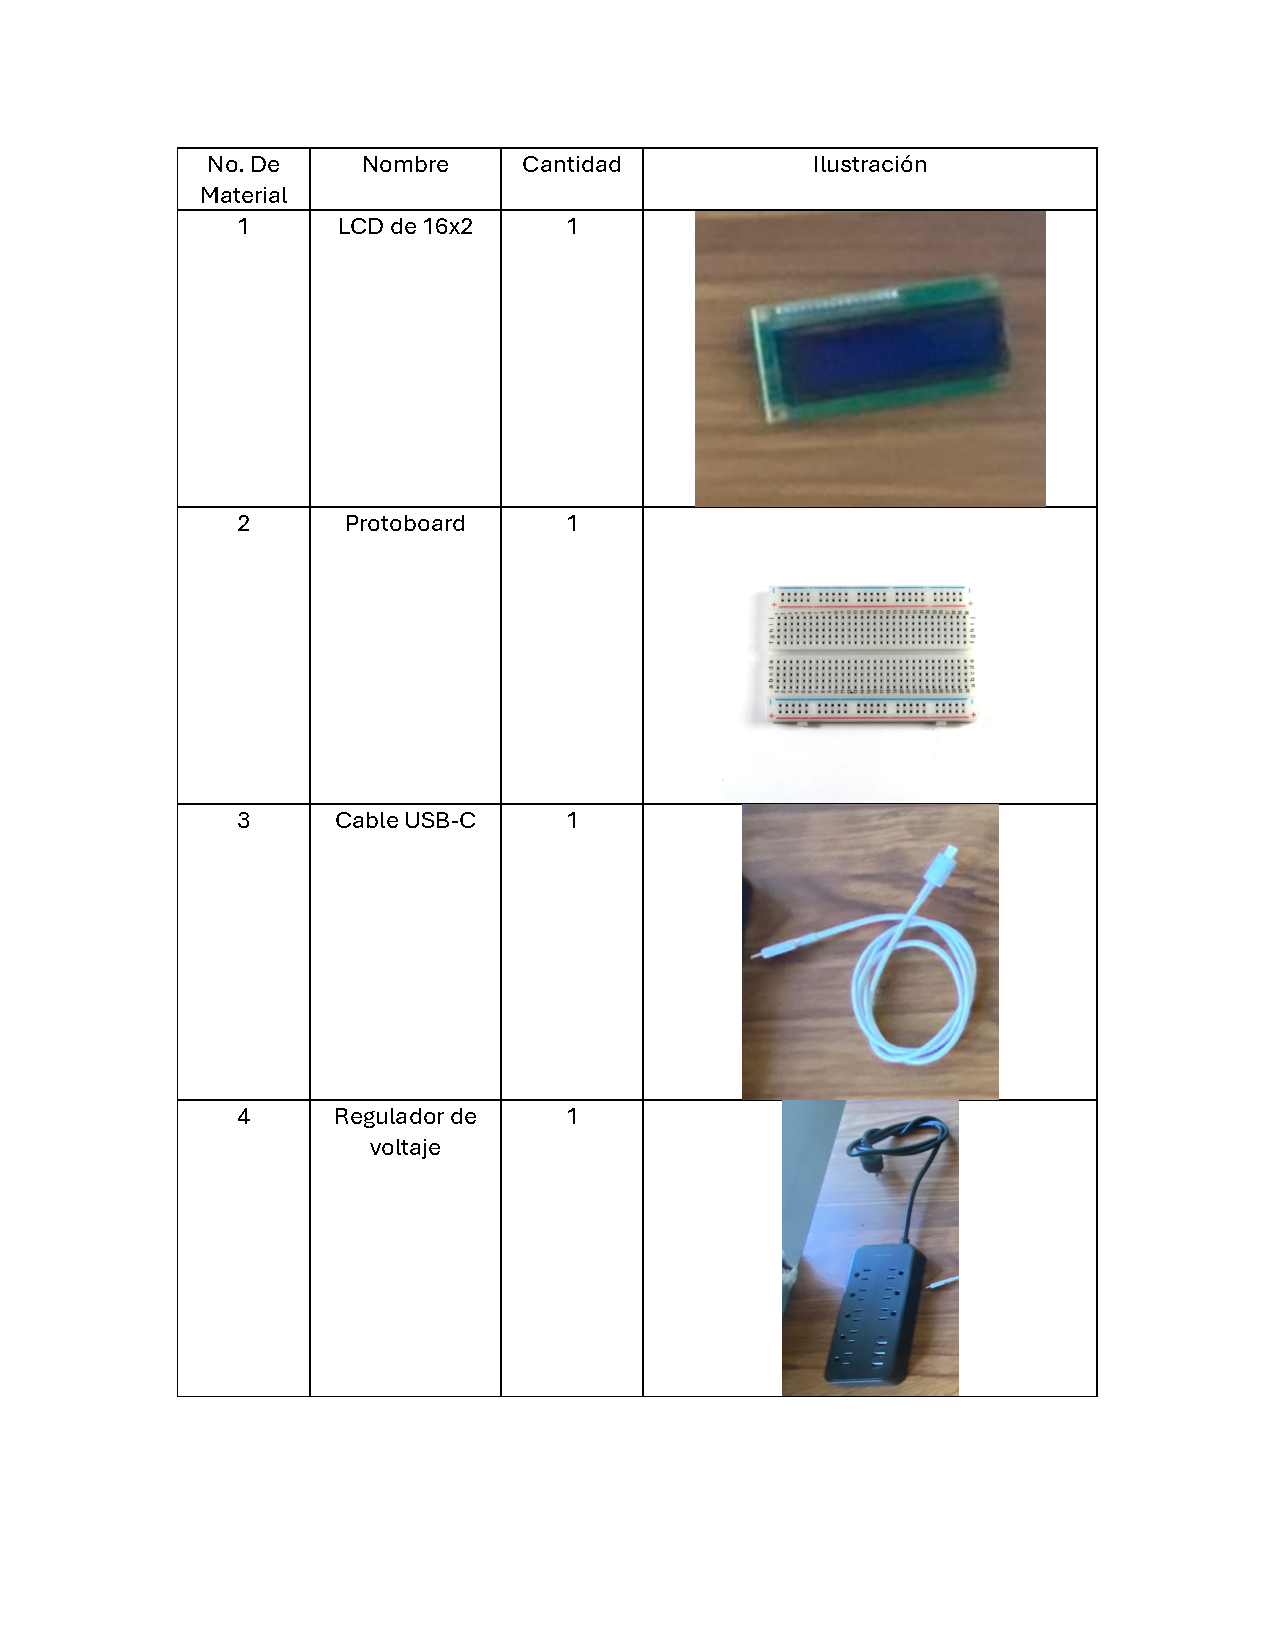
\includepdf[pages=-]{15/img/listaDeMateriales.pdf}
        \label{anexo:listaDeMateriales.pdf}

    %PZ-01
        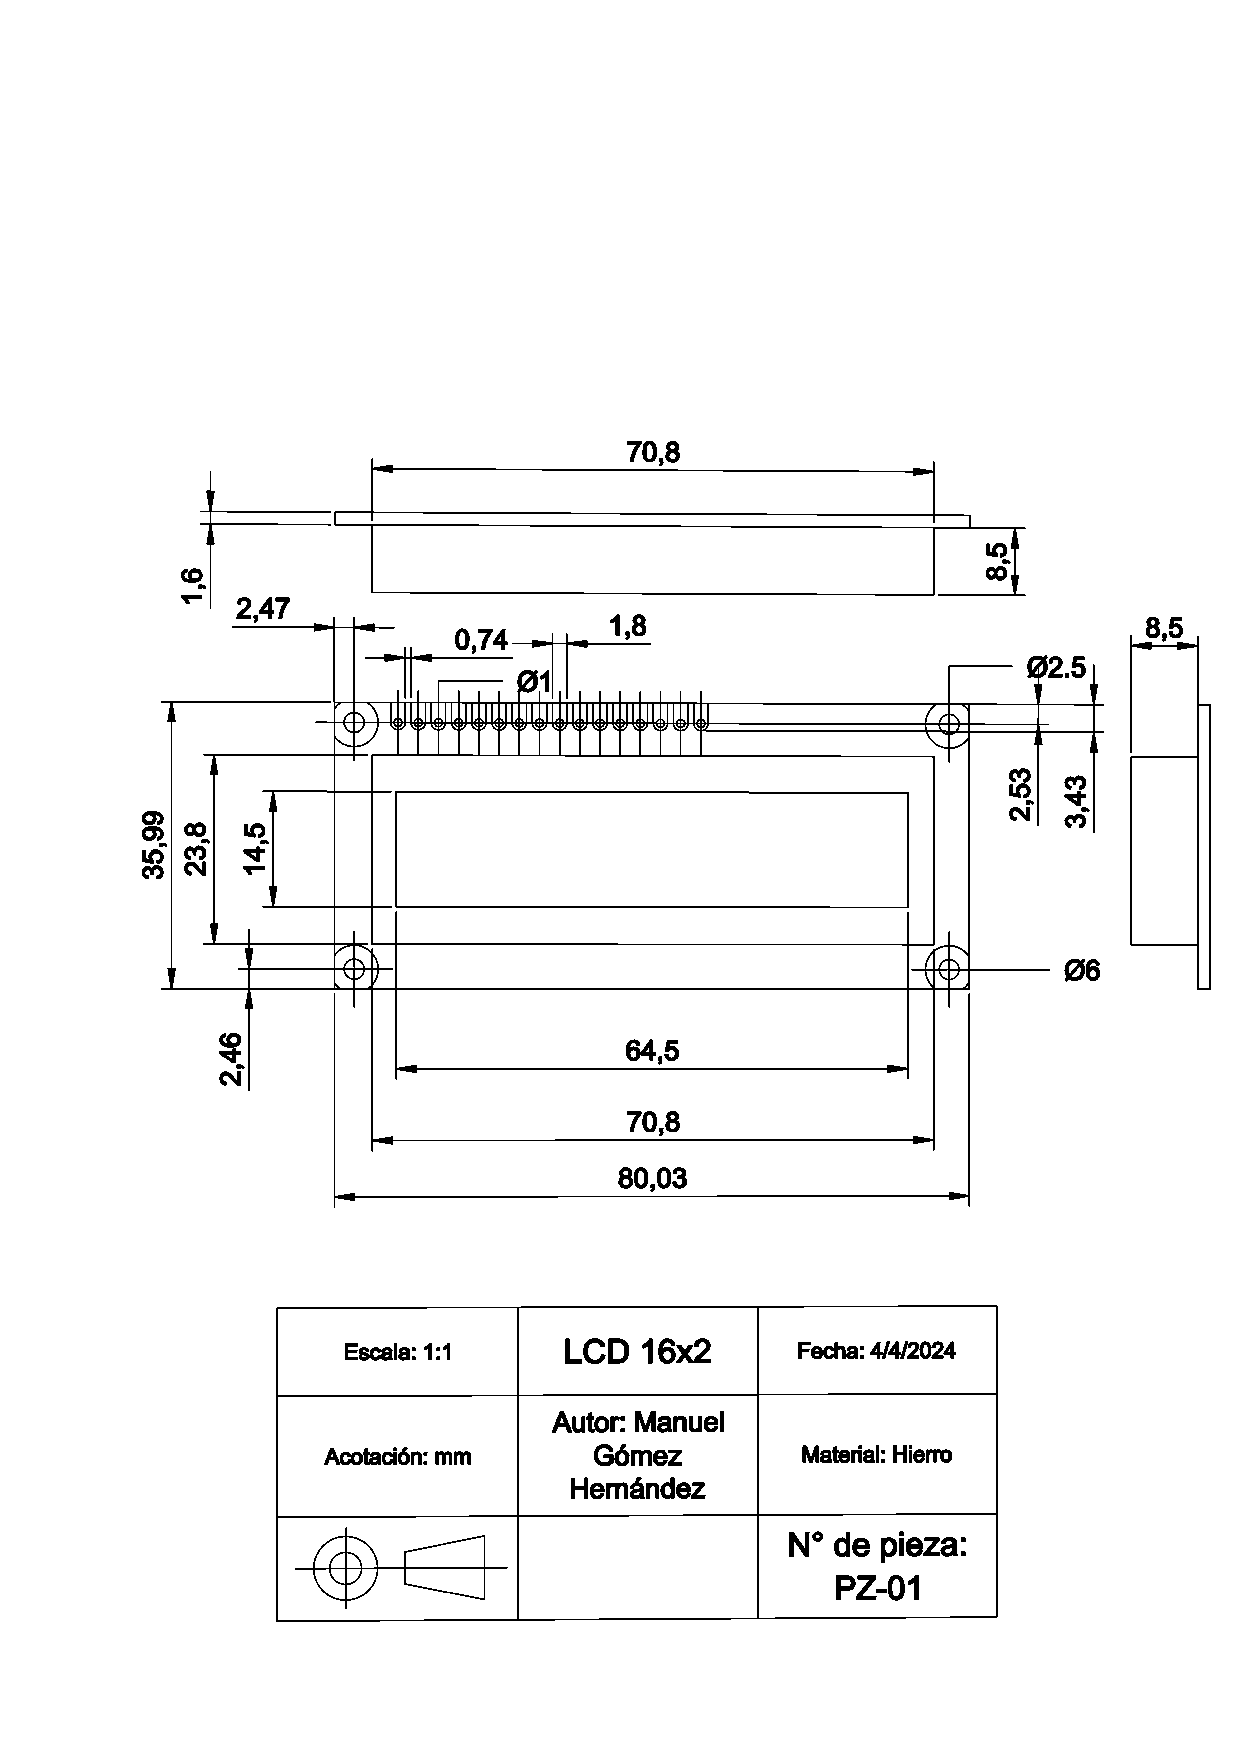
\includepdf[pages=-]{15/img/lcdTrazo.pdf}
        \label{anexo:lcdTrazo.pdf}
    
        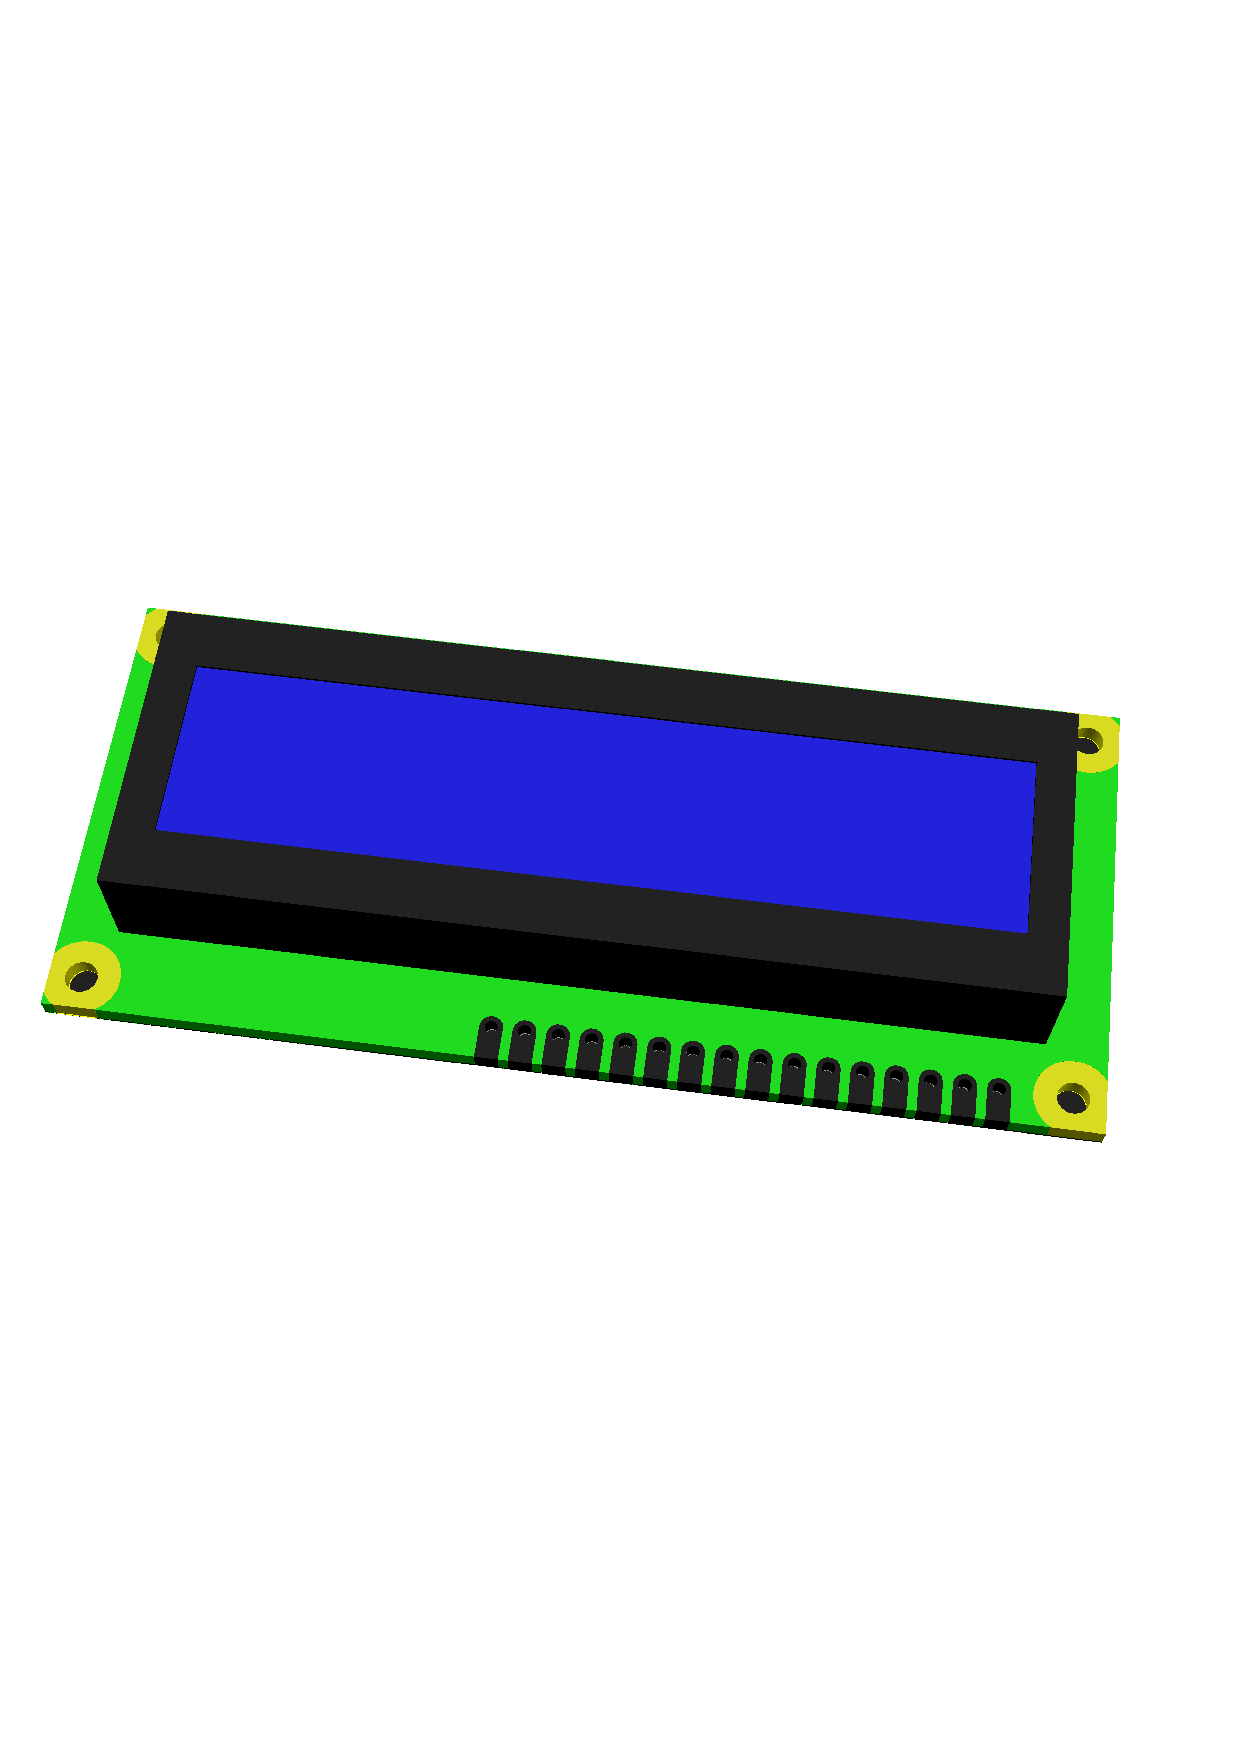
\includepdf[pages=-]{15/img/lcdModelo.pdf}
        \label{anexo:lcdModelo.pdf}
    %PZ-02
        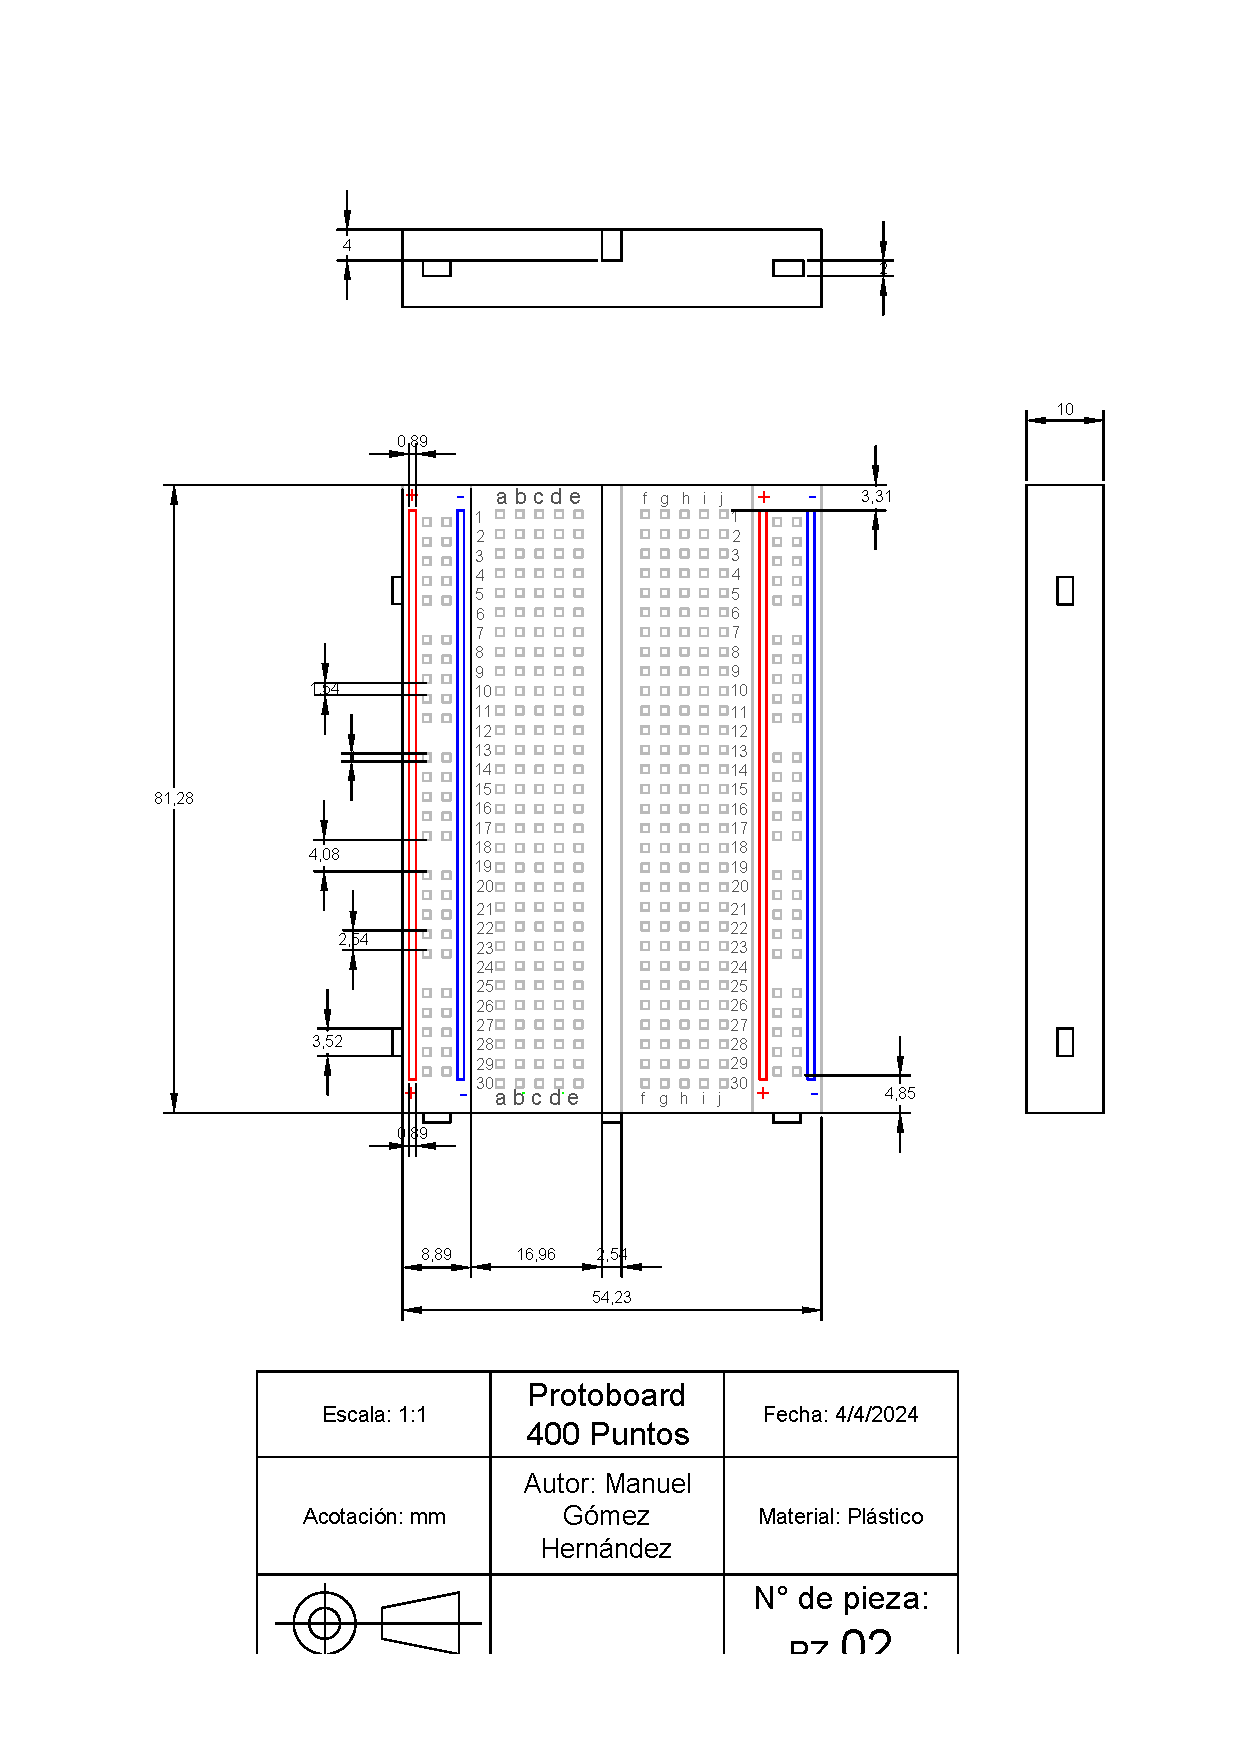
\includepdf[pages=-]{15/img/placaProtoboardTrazo.pdf}
        \label{anexo:placaProtoboardTrazo.pdf}
        
        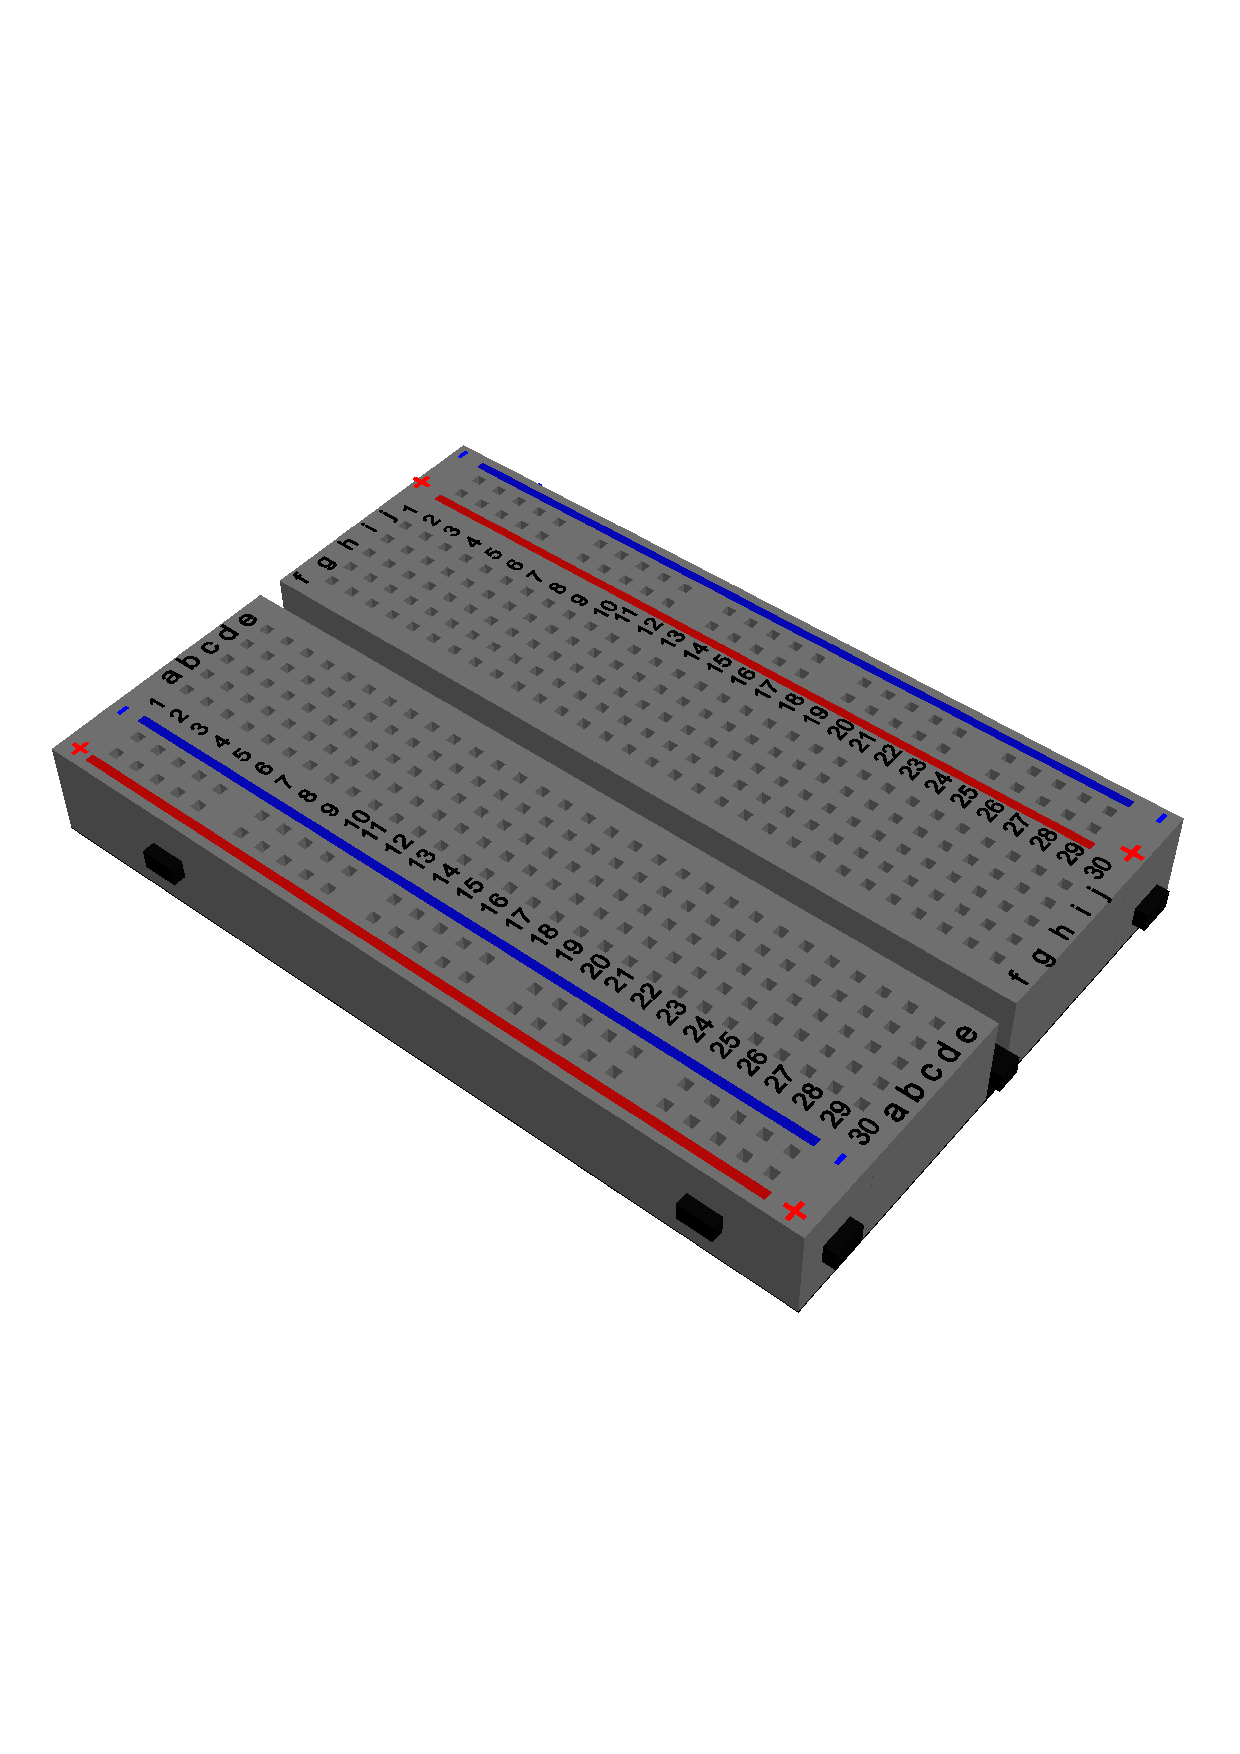
\includepdf[pages=-]{15/img/placaProtoboardModelo.pdf}
        \label{anexo:placaProtoboardModelo.pdf}
    %PZ-03
        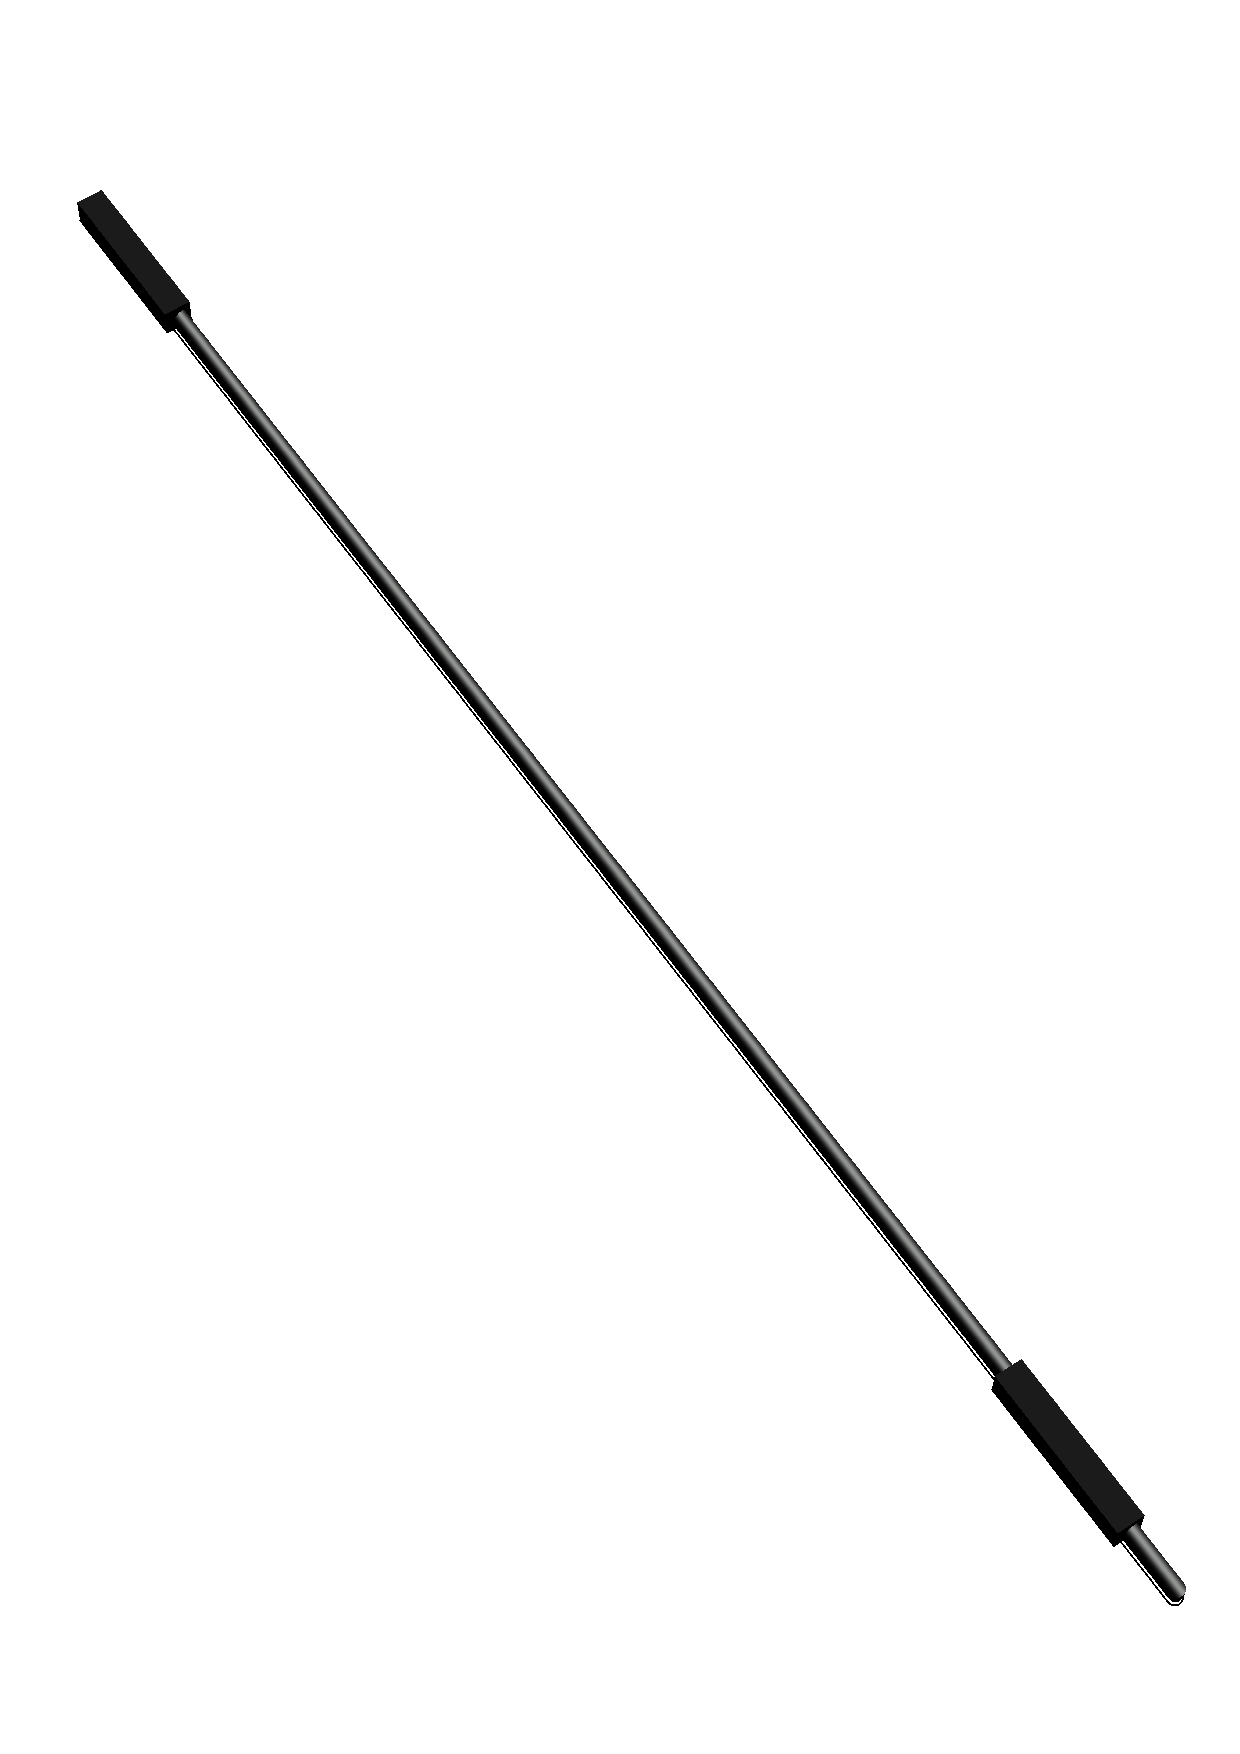
\includepdf[pages=-]{15/img/cableJumperMHModelo.pdf}
        \label{anexo:cableJumperMHModelo.pdf}
    
        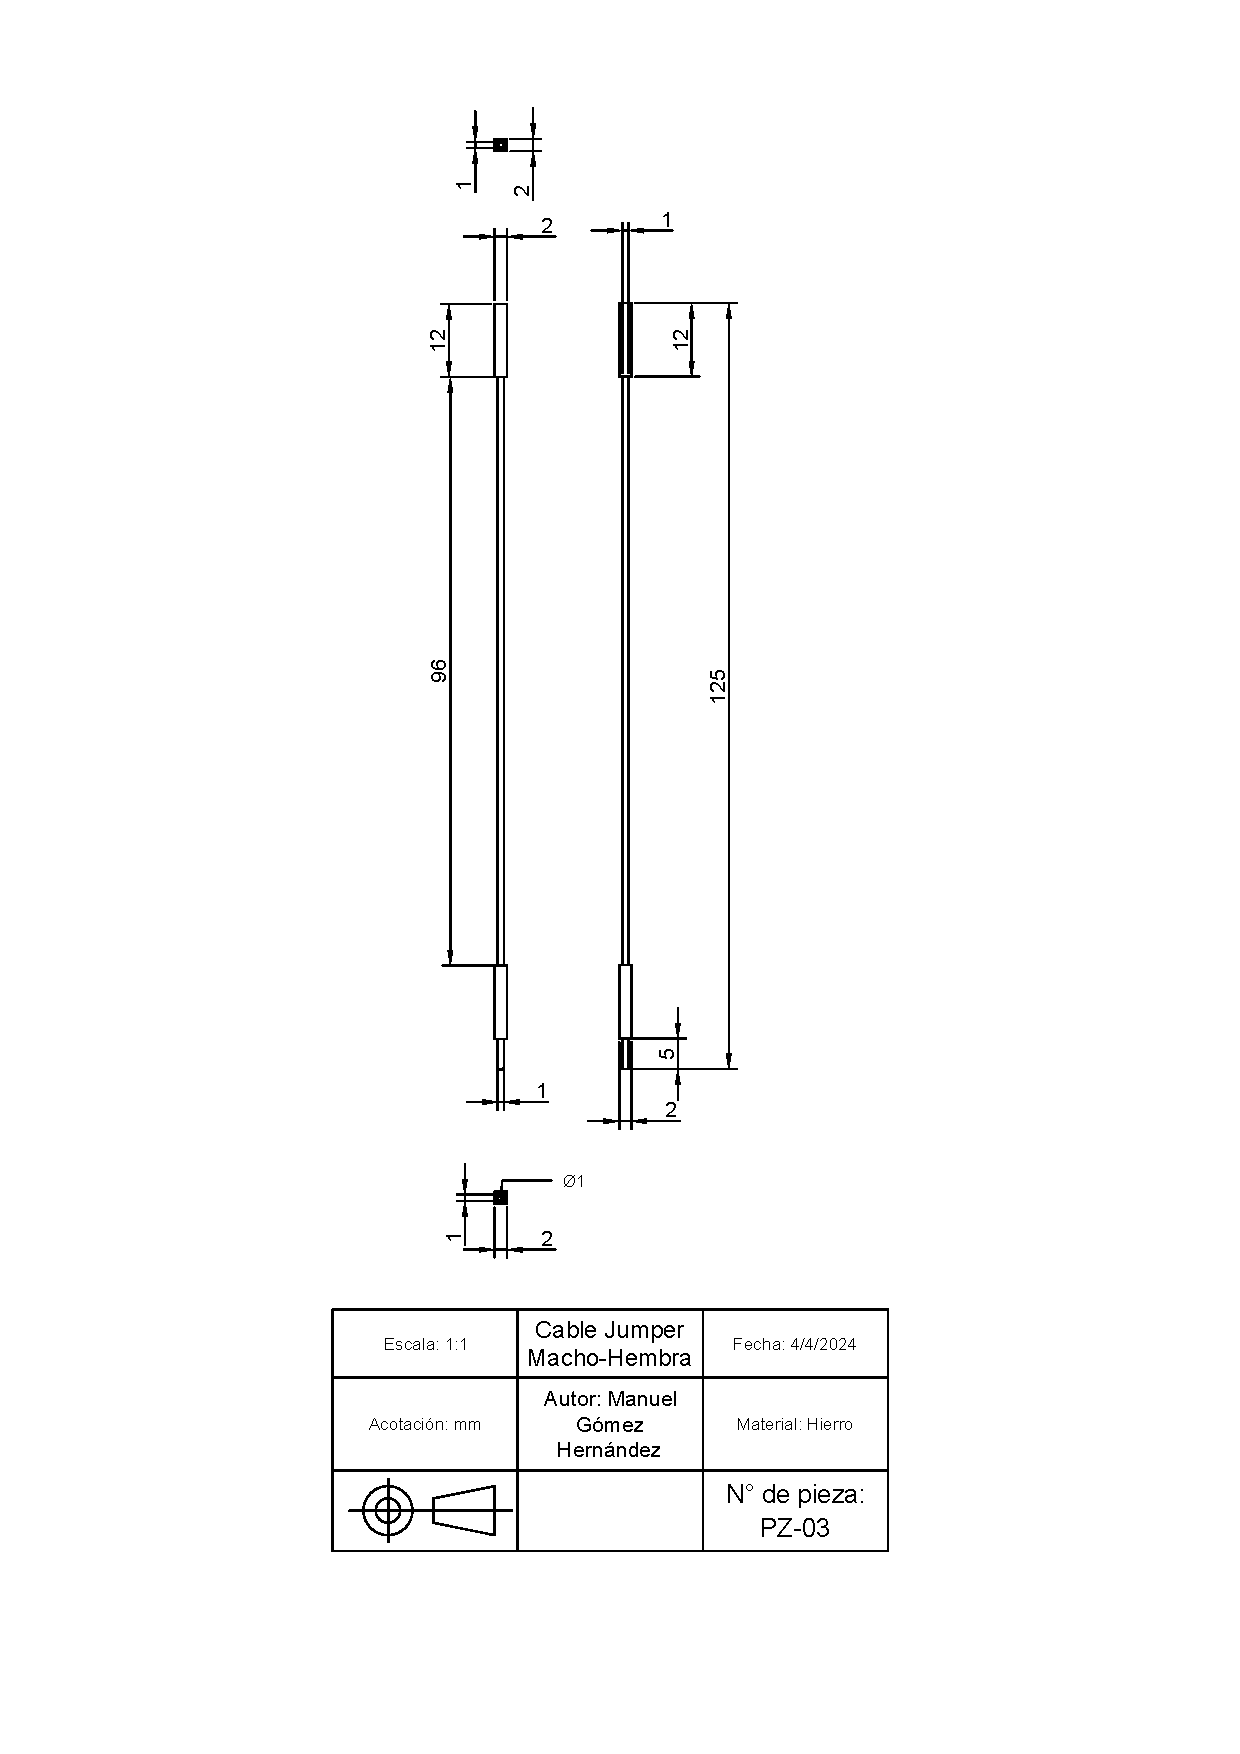
\includepdf[pages=-]{15/img/cableJumperMHTrazo.pdf}
        \label{anexo:cableJumperMHTrazo.pdf}
    %PZ-04
        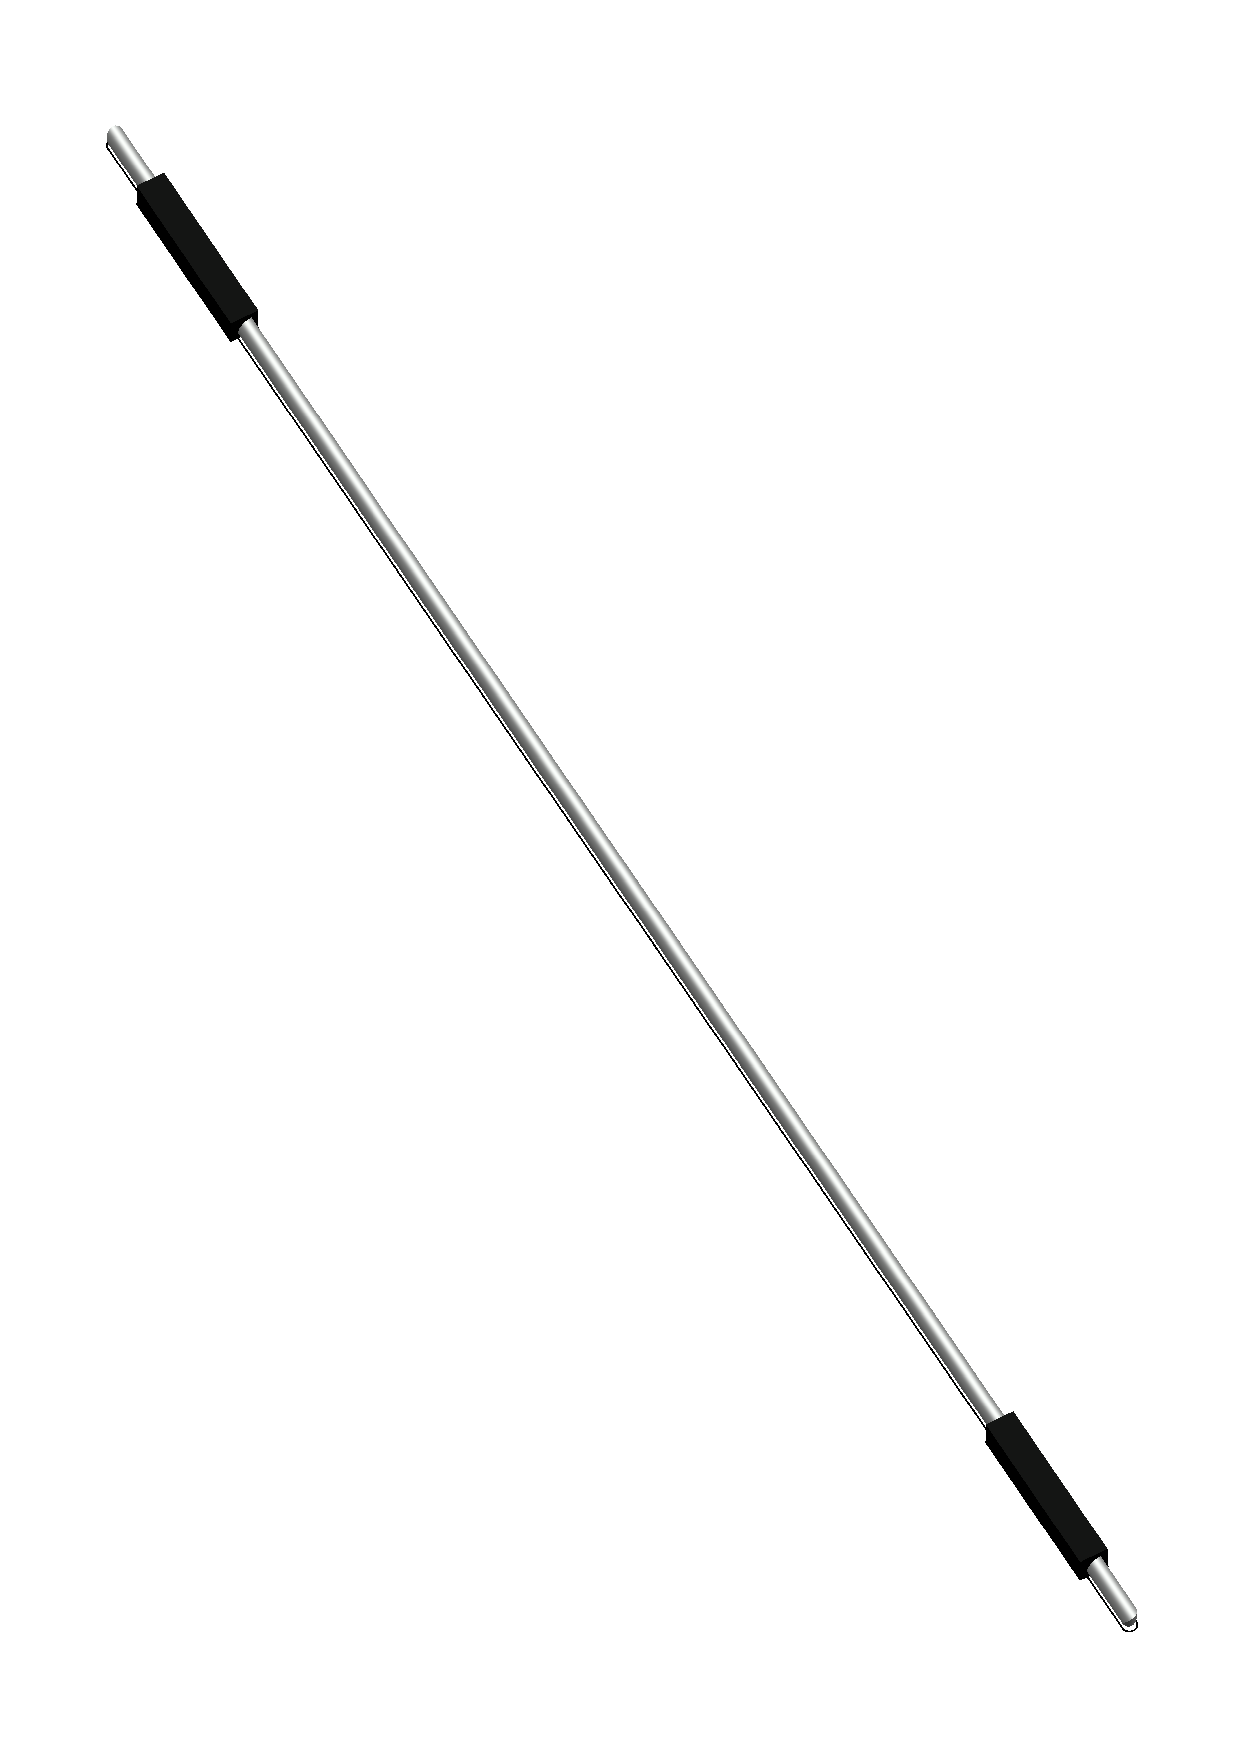
\includepdf[pages=-]{15/img/cableJumperMMModelo.pdf}
        \label{anexo:cableJumperMMModelo.pdf}
    
        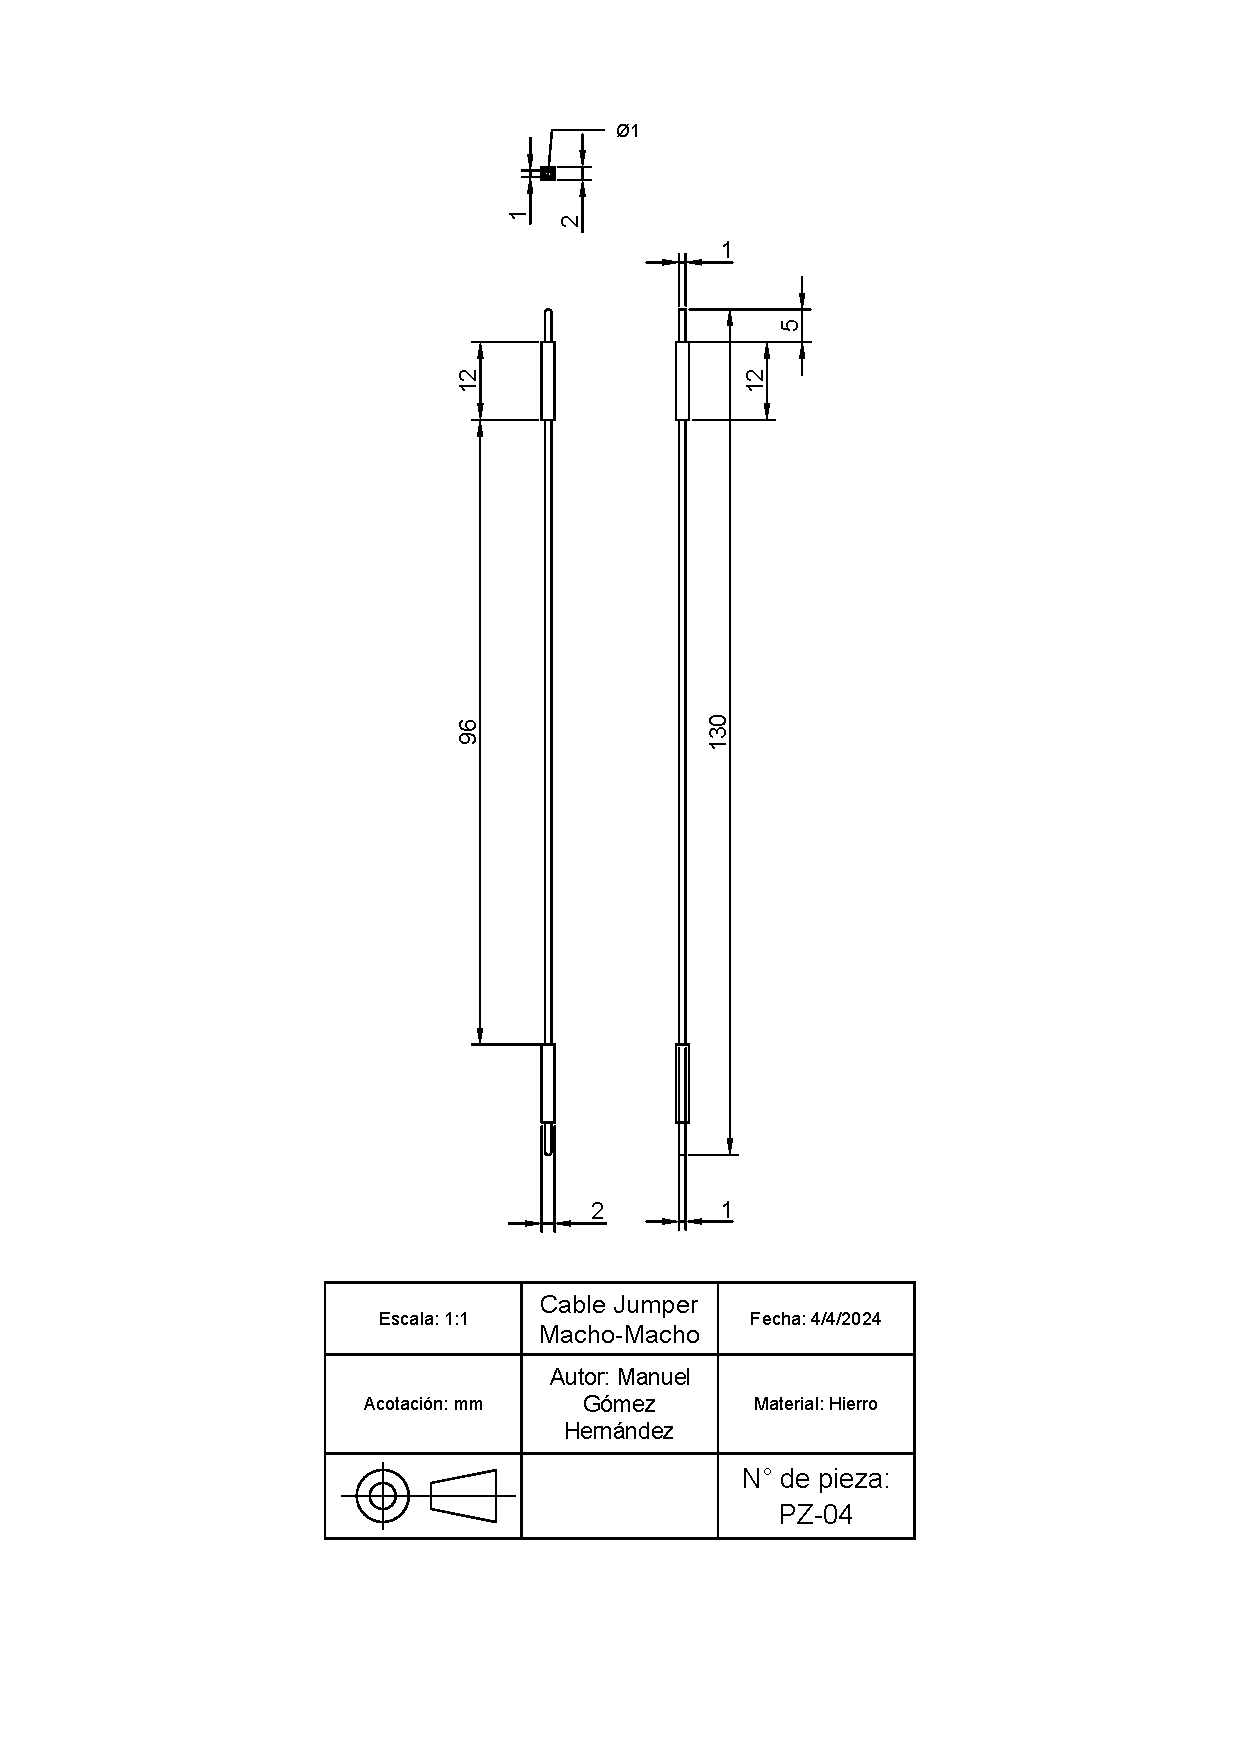
\includepdf[pages=-]{15/img/cableJumperMMTrazo.pdf}
        \label{anexo:cableJumperMMTrazo.pdf}
    %PZ-05
        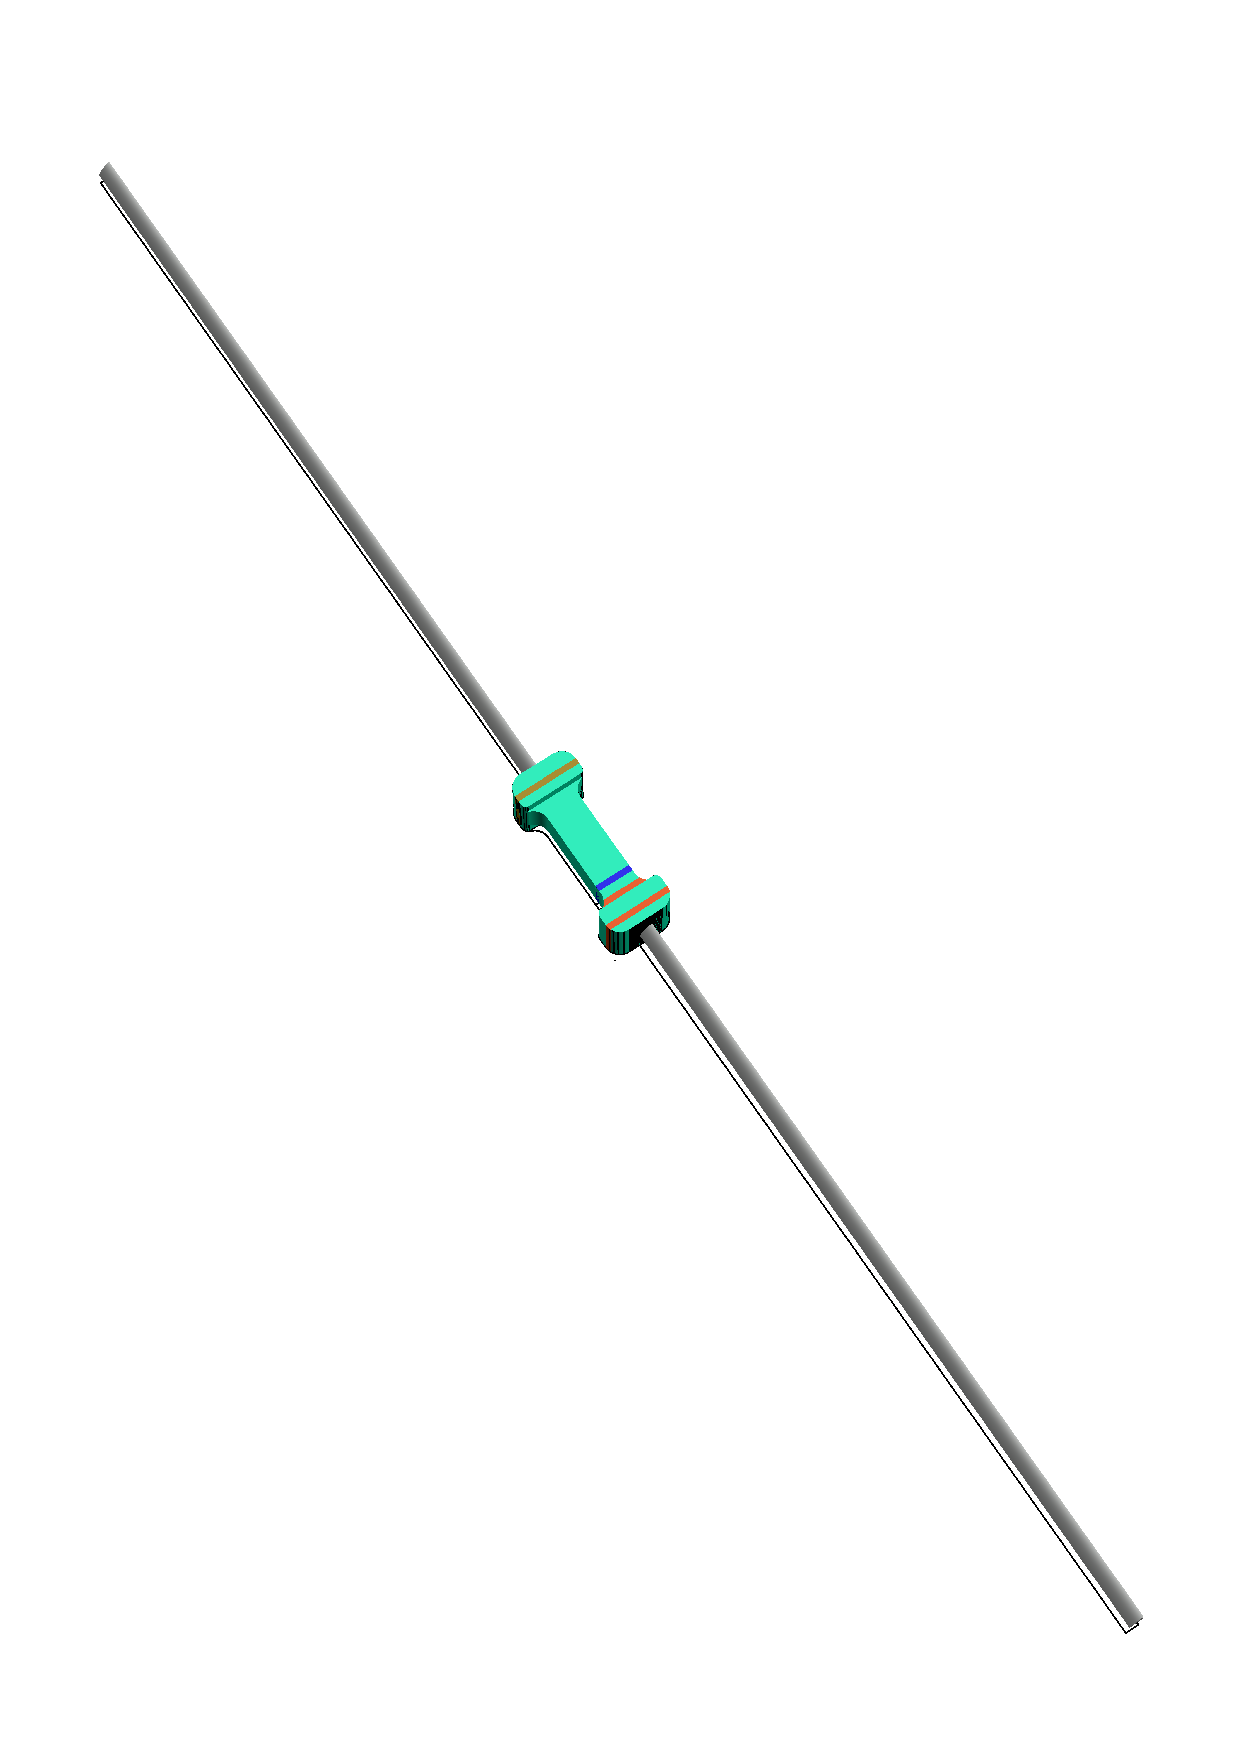
\includepdf[pages=-]{15/img/resistenciaModelo.pdf}
        \label{anexo:resistenciaModelo.pdf}
    
        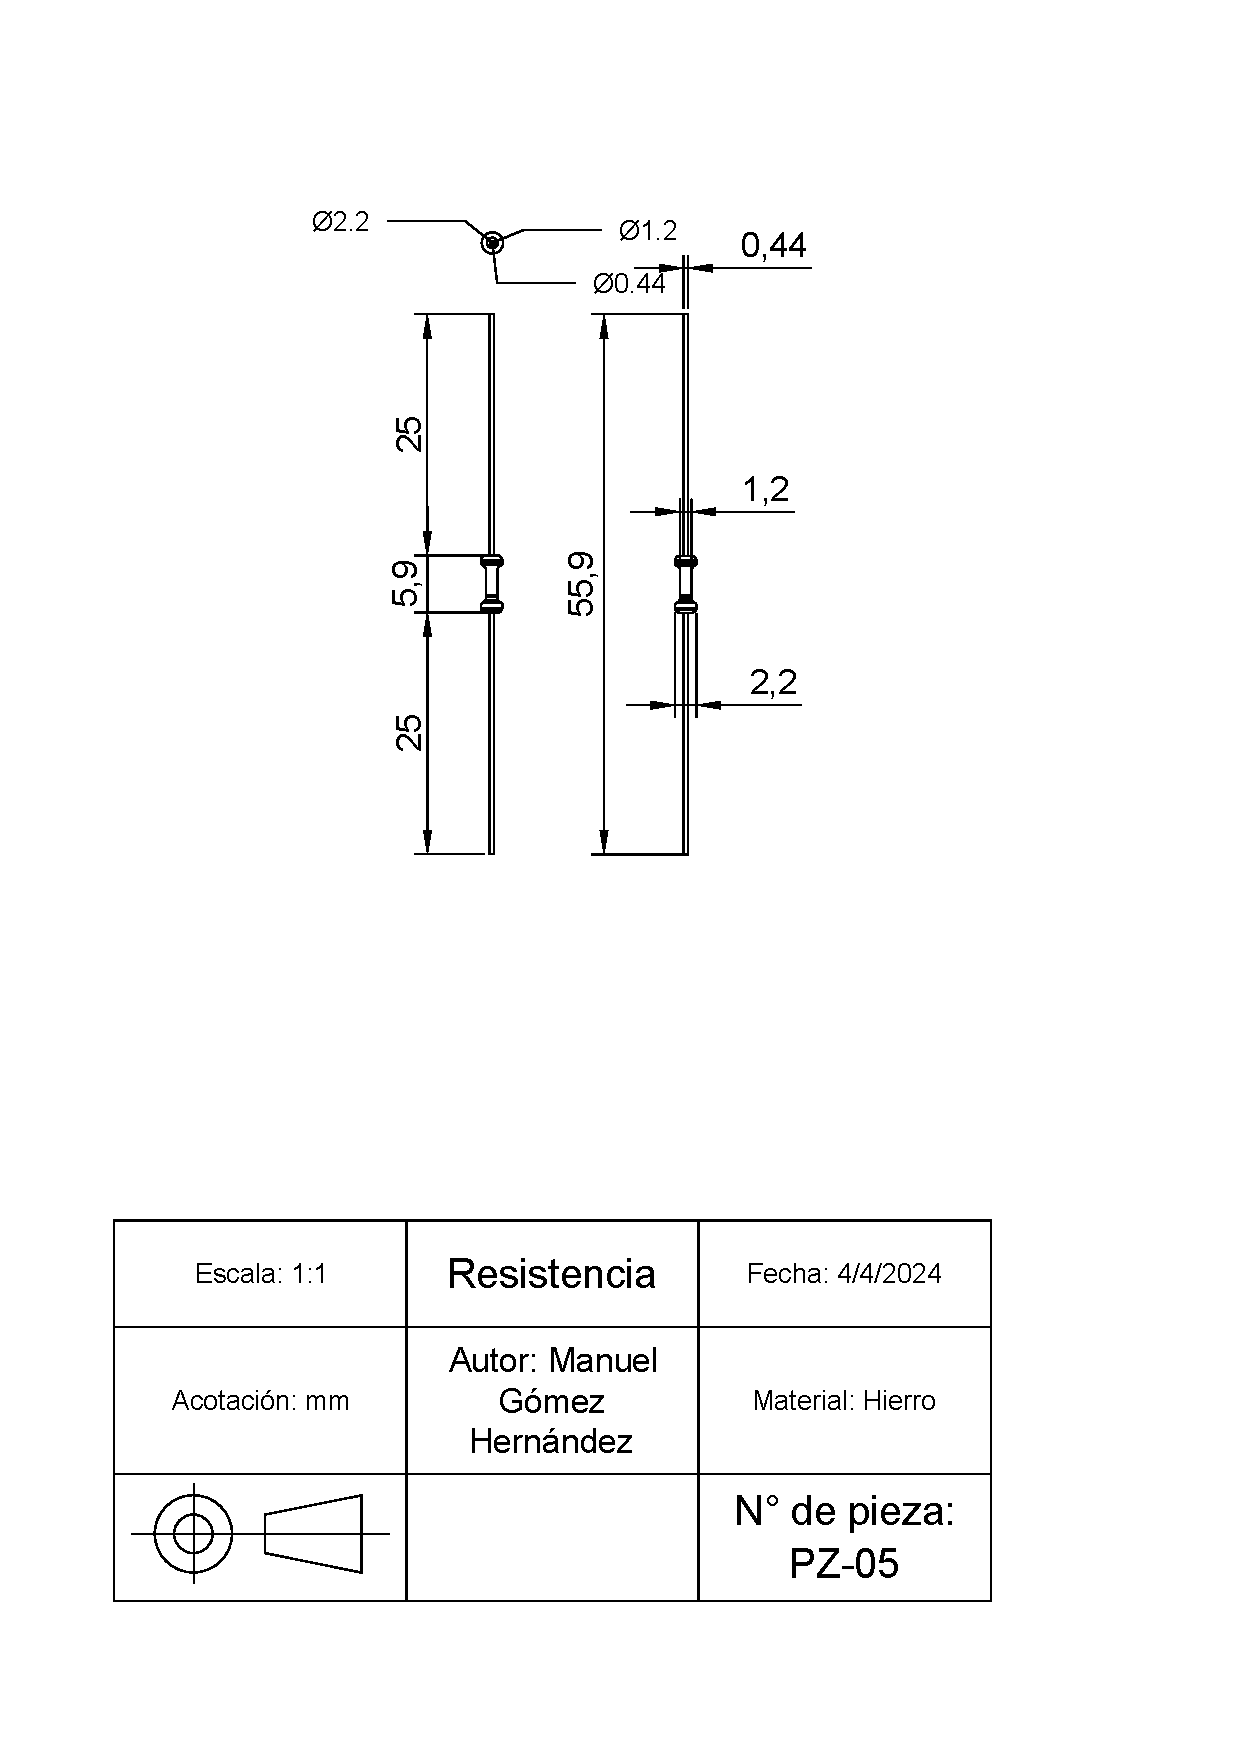
\includepdf[pages=-]{15/img/resistenciaTrazo.pdf}
        \label{anexo:resistenciaTrazo.pdf}
    %PZ-06
        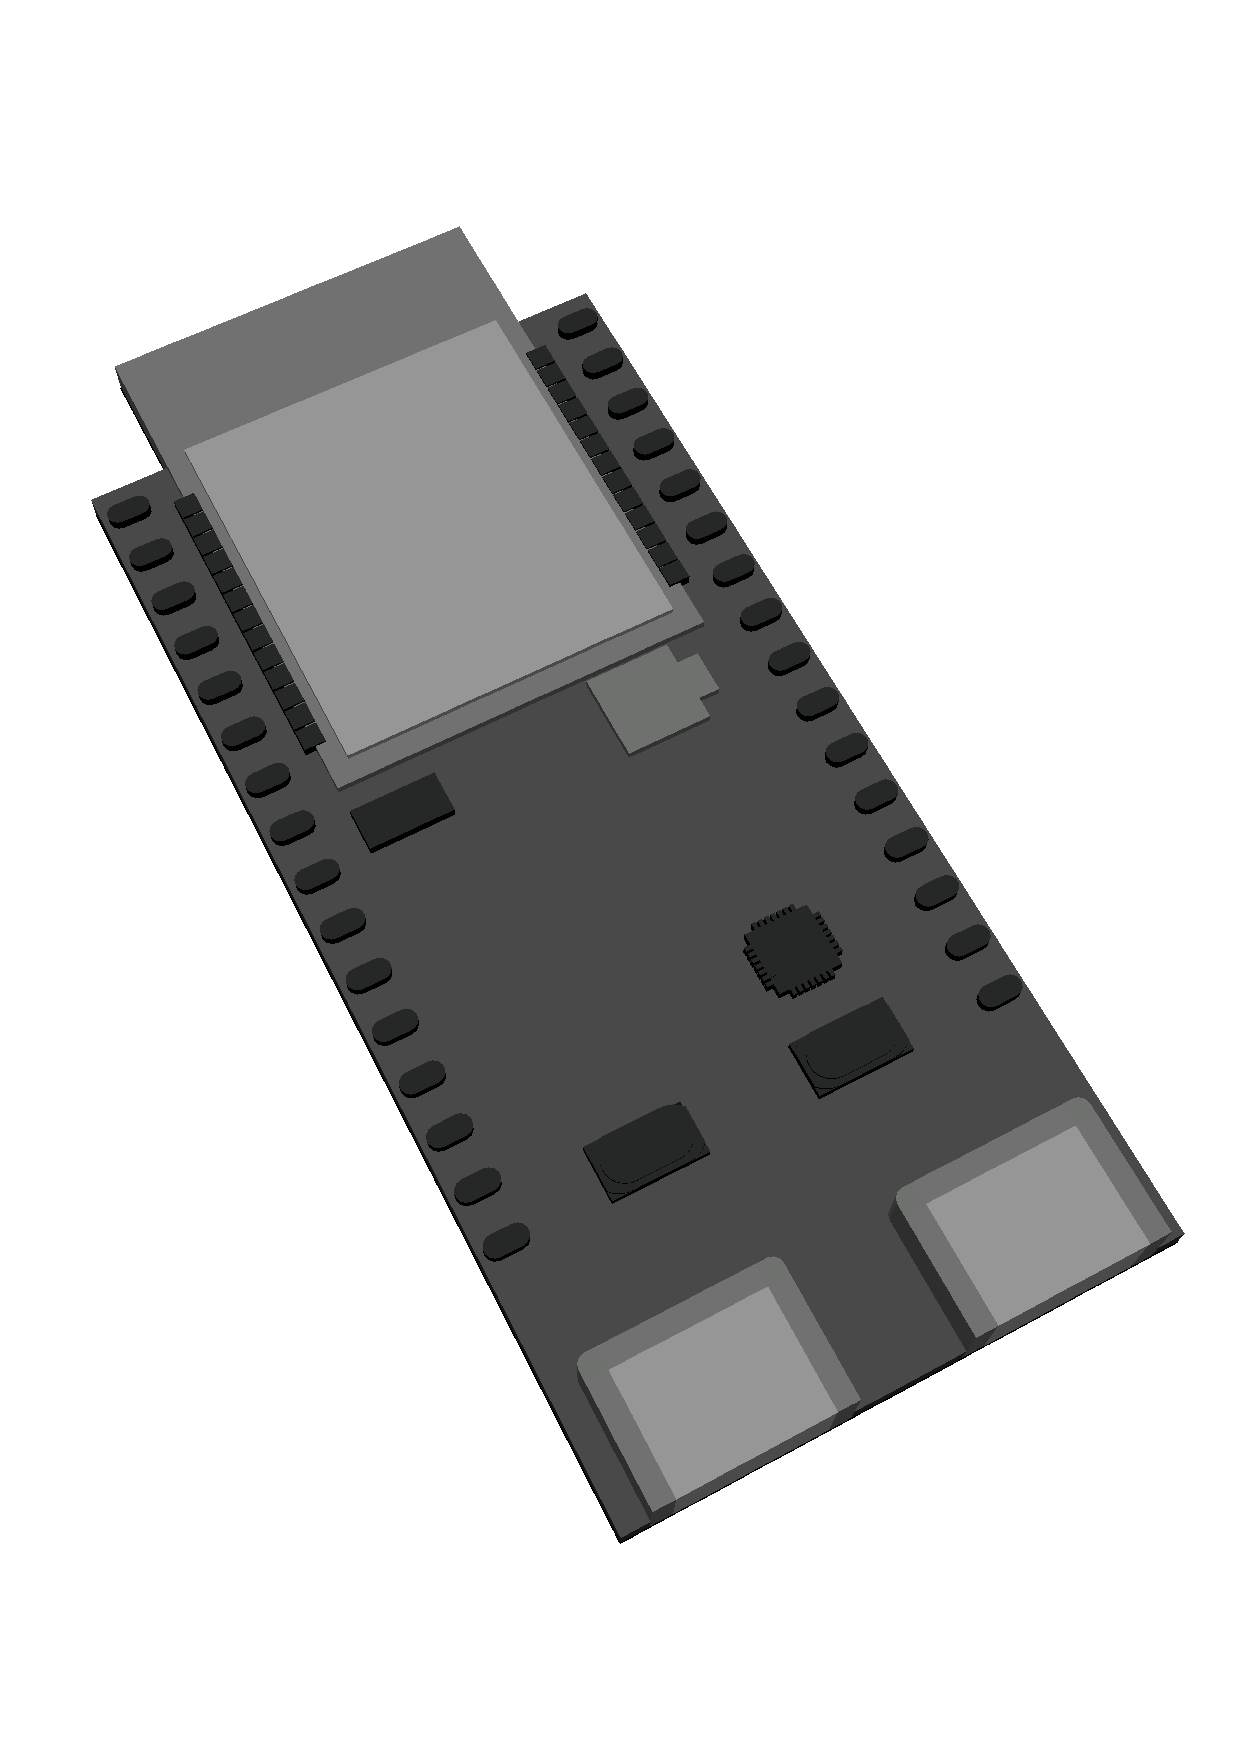
\includepdf[pages=-]{15/img/eSP32Modelo.pdf}
        \label{anexo:eSP32Modelo.pdf}
    
        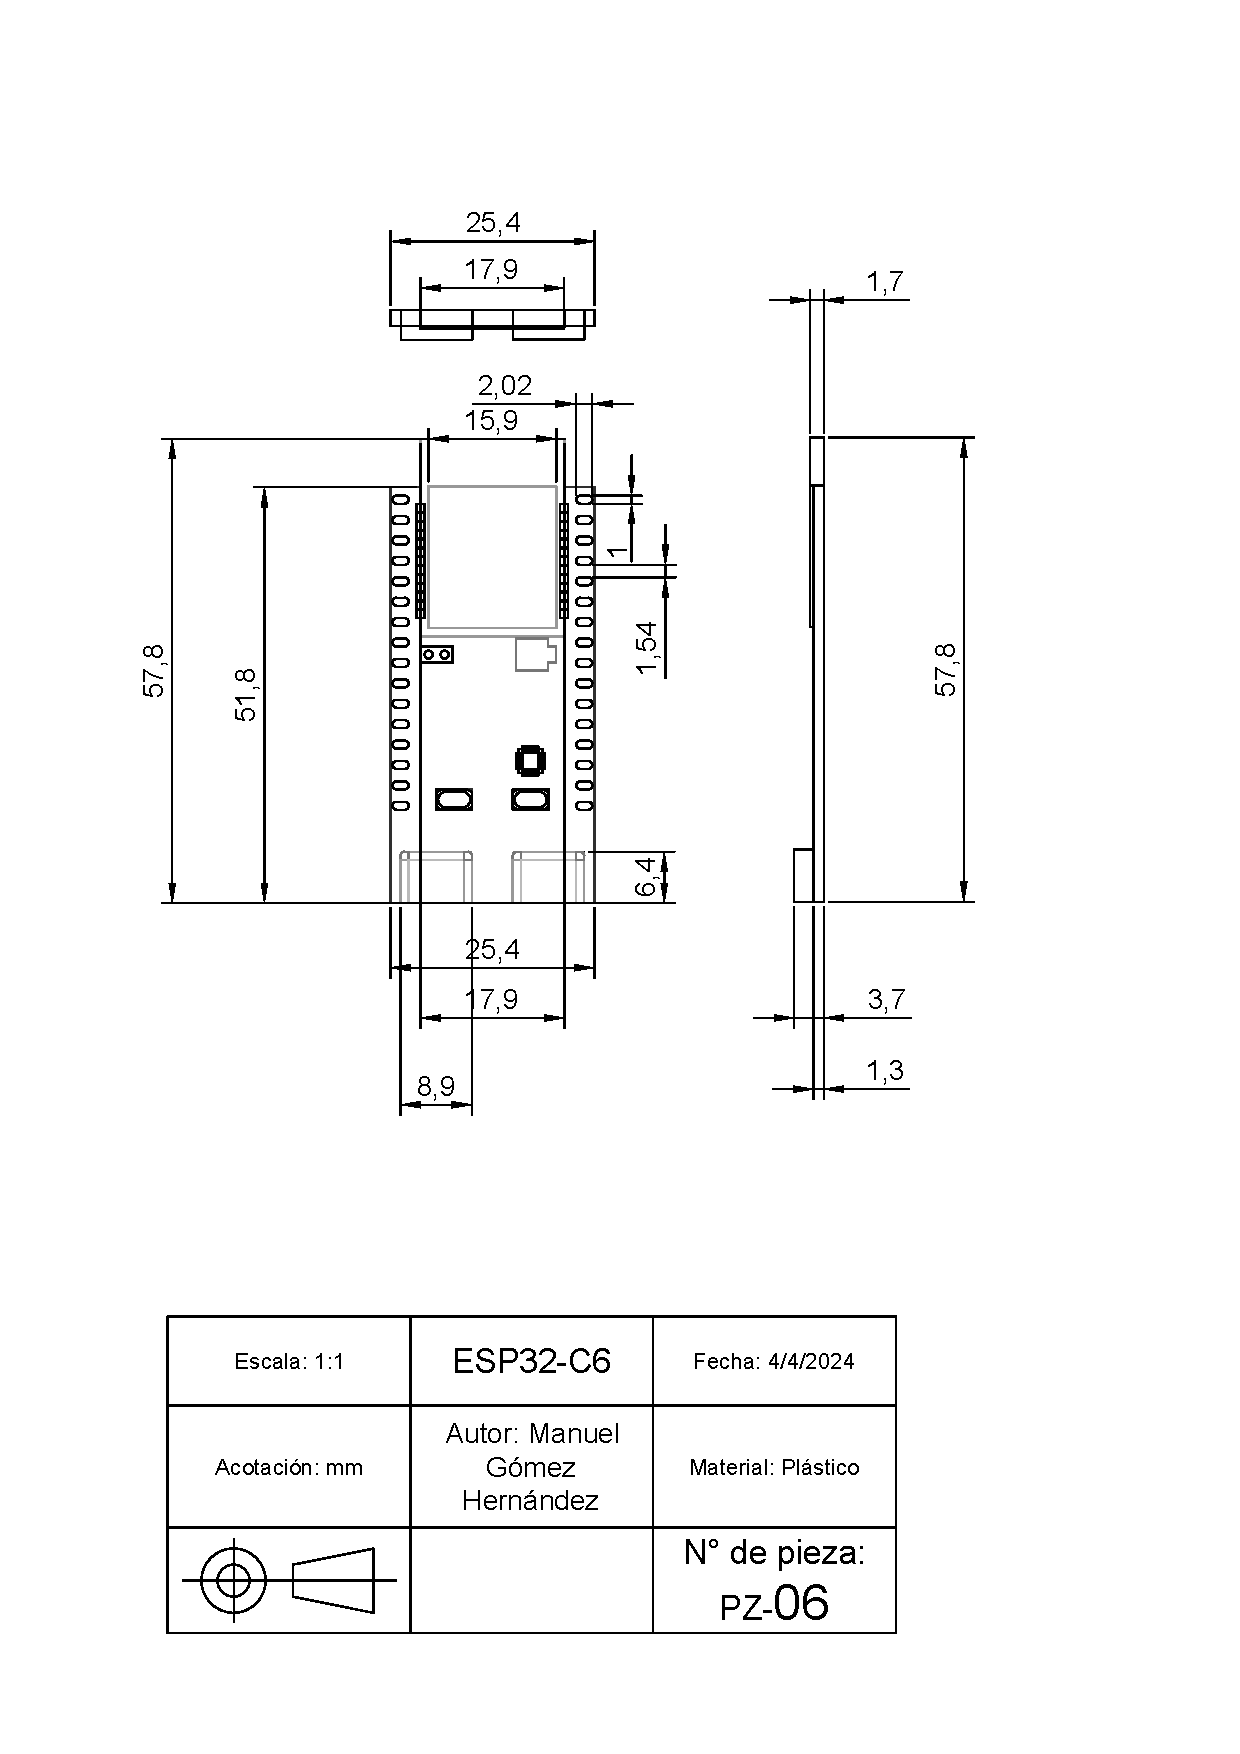
\includepdf[pages=-]{15/img/eSP32Trazo.pdf}
        \label{anexo:eSP32Trazo.pdf}
    %PZ-07
        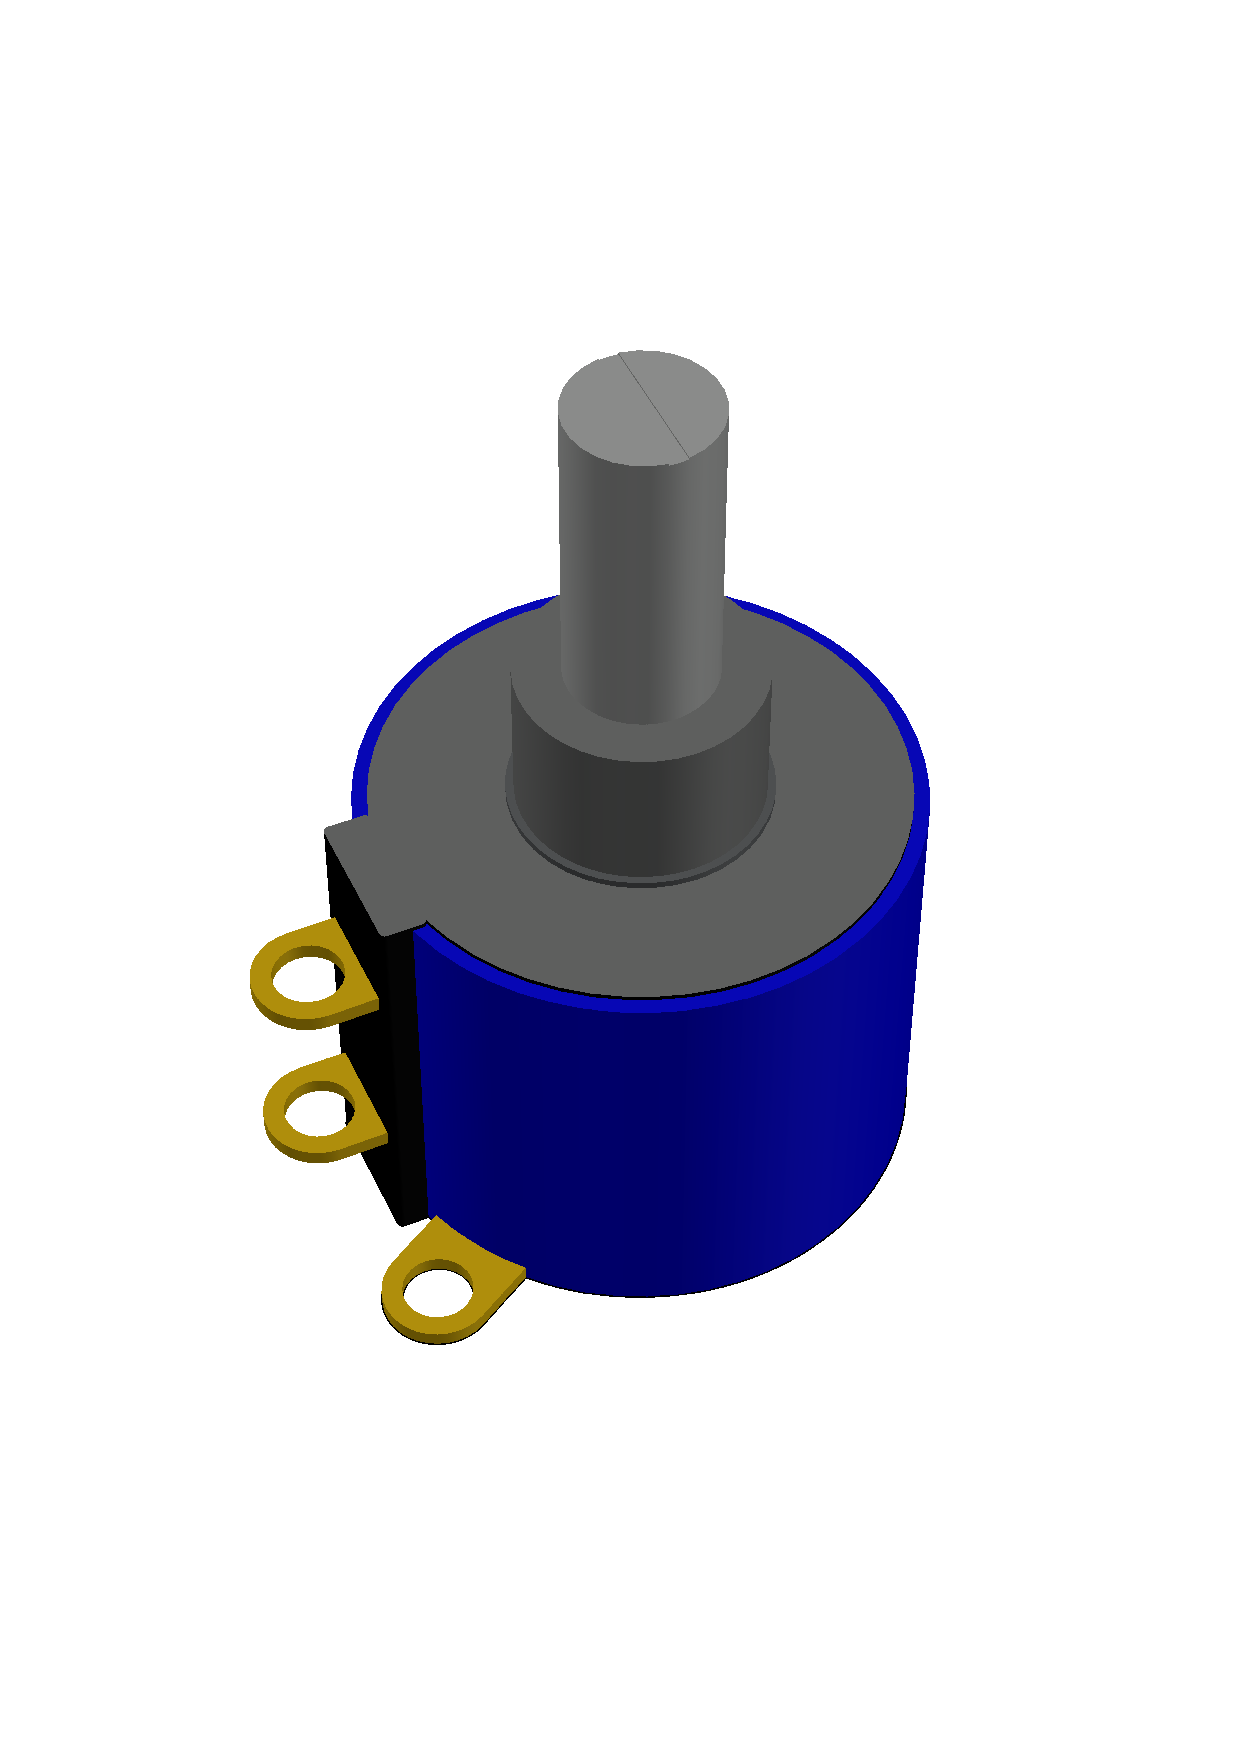
\includepdf[pages=-]{15/img/potenciometroModelo.pdf}
        \label{anexo:potenciometroModelo.pdf}
    
        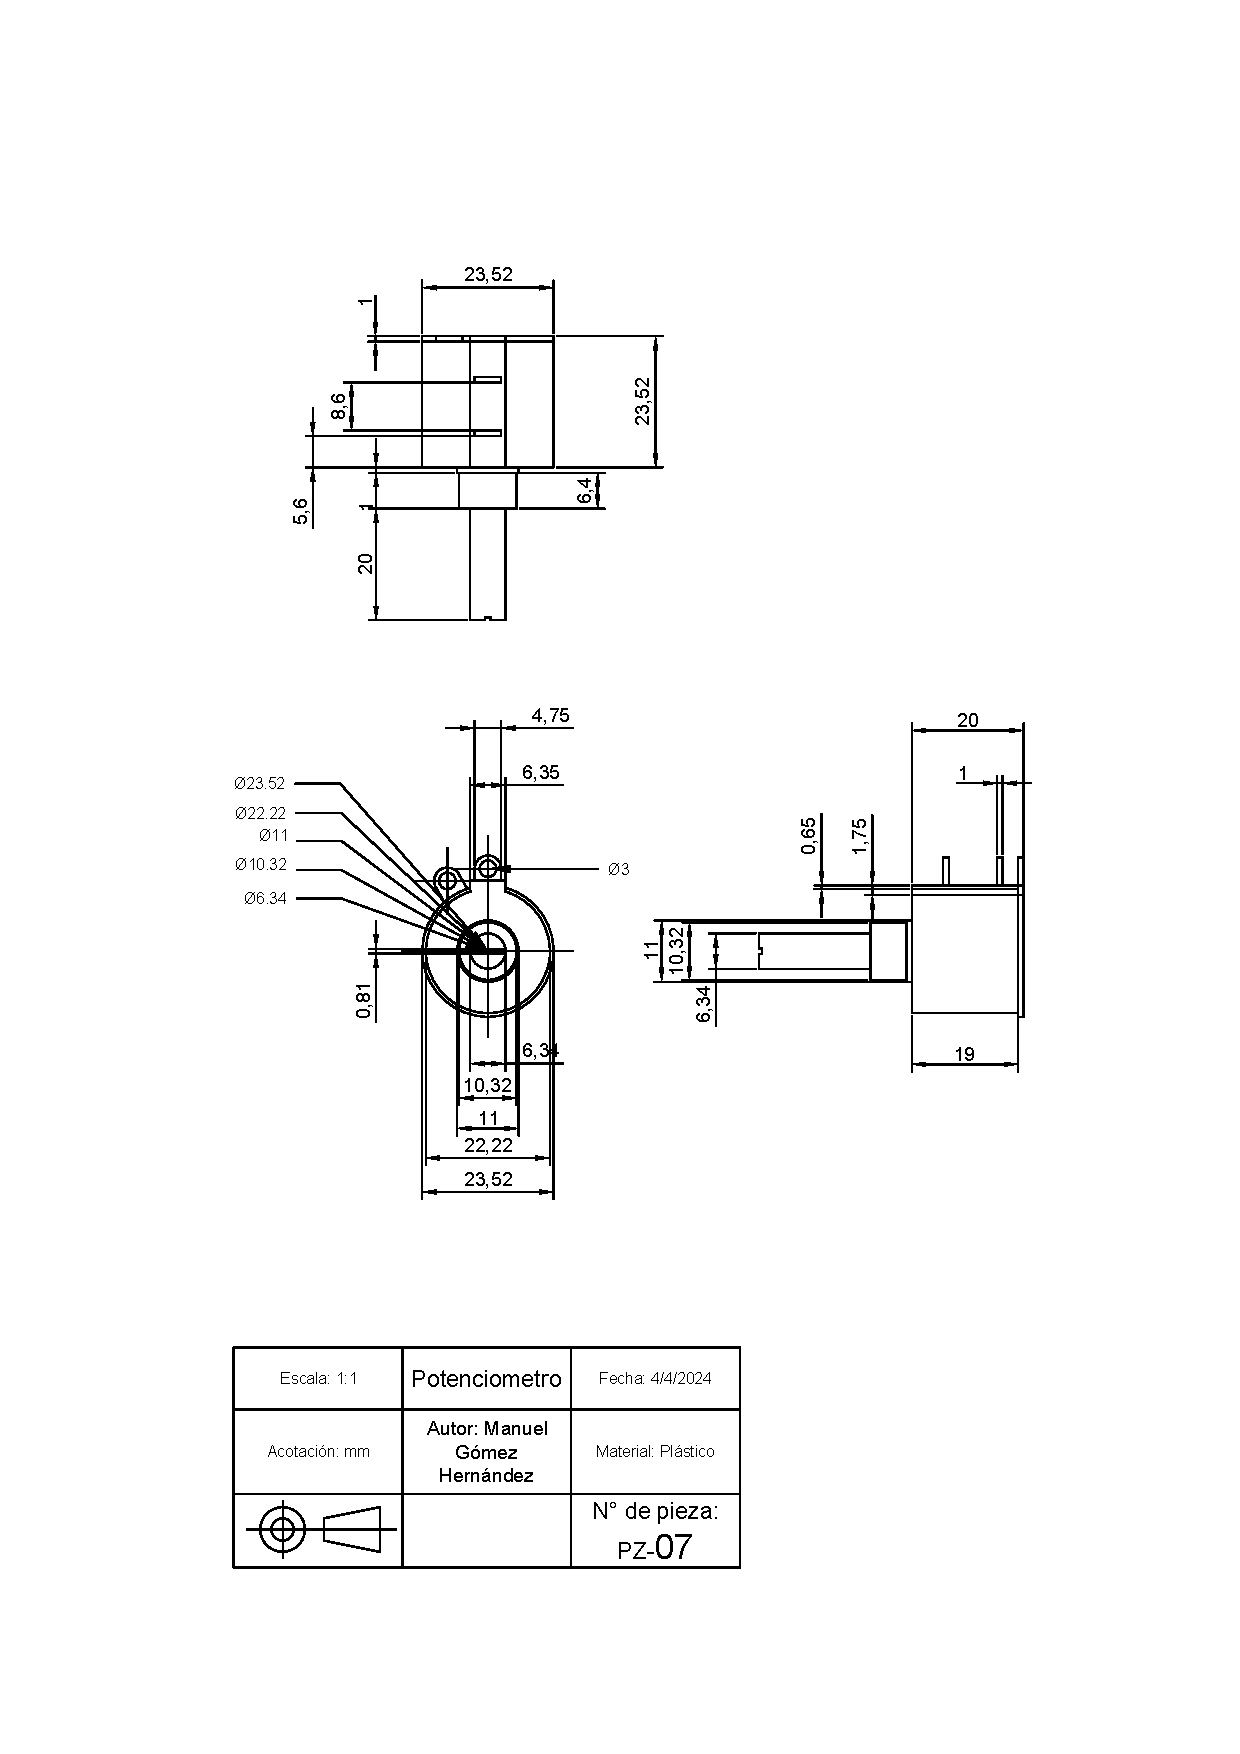
\includepdf[pages=-]{15/img/potenciometroTrazo.pdf}
        \label{anexo:potenciometroTrazo.pdf}
    %PZ-08
        %\includepdf[pages=-]{15/img/manualDeEnsambleDeCircuitoElectronicoEsp32-c6.pdf}
        %\label{anexo:manualDeEnsambleDeCircuitoElectronicoEsp32-c6.pdf}
    
        %\includepdf[pages=-]{15/img/manualDeEnsambleDeCircuitoElectronicoEsp32-c6.pdf}
        %\label{anexo:manualDeEnsambleDeCircuitoElectronicoEsp32-c6.pdf}
    %PZ-09
        %\includepdf[pages=-]{15/img/manualDeEnsambleDeCircuitoElectronicoEsp32-c6.pdf}
        %\label{anexo:manualDeEnsambleDeCircuitoElectronicoEsp32-c6.pdf}
    
        %\includepdf[pages=-]{15/img/manualDeEnsambleDeCircuitoElectronicoEsp32-c6.pdf}
        %\label{anexo:manualDeEnsambleDeCircuitoElectronicoEsp32-c6.pdf}
    %PZ-10
        %\includepdf[pages=-]{15/img/manualDeEnsambleDeCircuitoElectronicoEsp32-c6.pdf}
        %\label{anexo:manualDeEnsambleDeCircuitoElectronicoEsp32-c6.pdf}
    
        %\includepdf[pages=-]{15/img/manualDeEnsambleDeCircuitoElectronicoEsp32-c6.pdf}
        %\label{anexo:manualDeEnsambleDeCircuitoElectronicoEsp32-c6.pdf}
    %PZ-11
        %\includepdf[pages=-]{15/img/manualDeEnsambleDeCircuitoElectronicoEsp32-c6.pdf}
       % \label{anexo:manualDeEnsambleDeCircuitoElectronicoEsp32-c6.pdf}
    
        %\includepdf[pages=-]{15/img/manualDeEnsambleDeCircuitoElectronicoEsp32-c6.pdf}
        %\label{anexo:manualDeEnsambleDeCircuitoElectronicoEsp32-c6.pdf}
    
    %Manual de ensabmble del circuito
        \includepdf[pages=-]{15/img/manualDeEnsambleDeCircuitoElectronicoEsp32-c6.pdf}
        \label{anexo:manualDeEnsambleDeCircuitoElectronicoEsp32-c6.pdf}


    %Hoja de registro del primer ensamble
    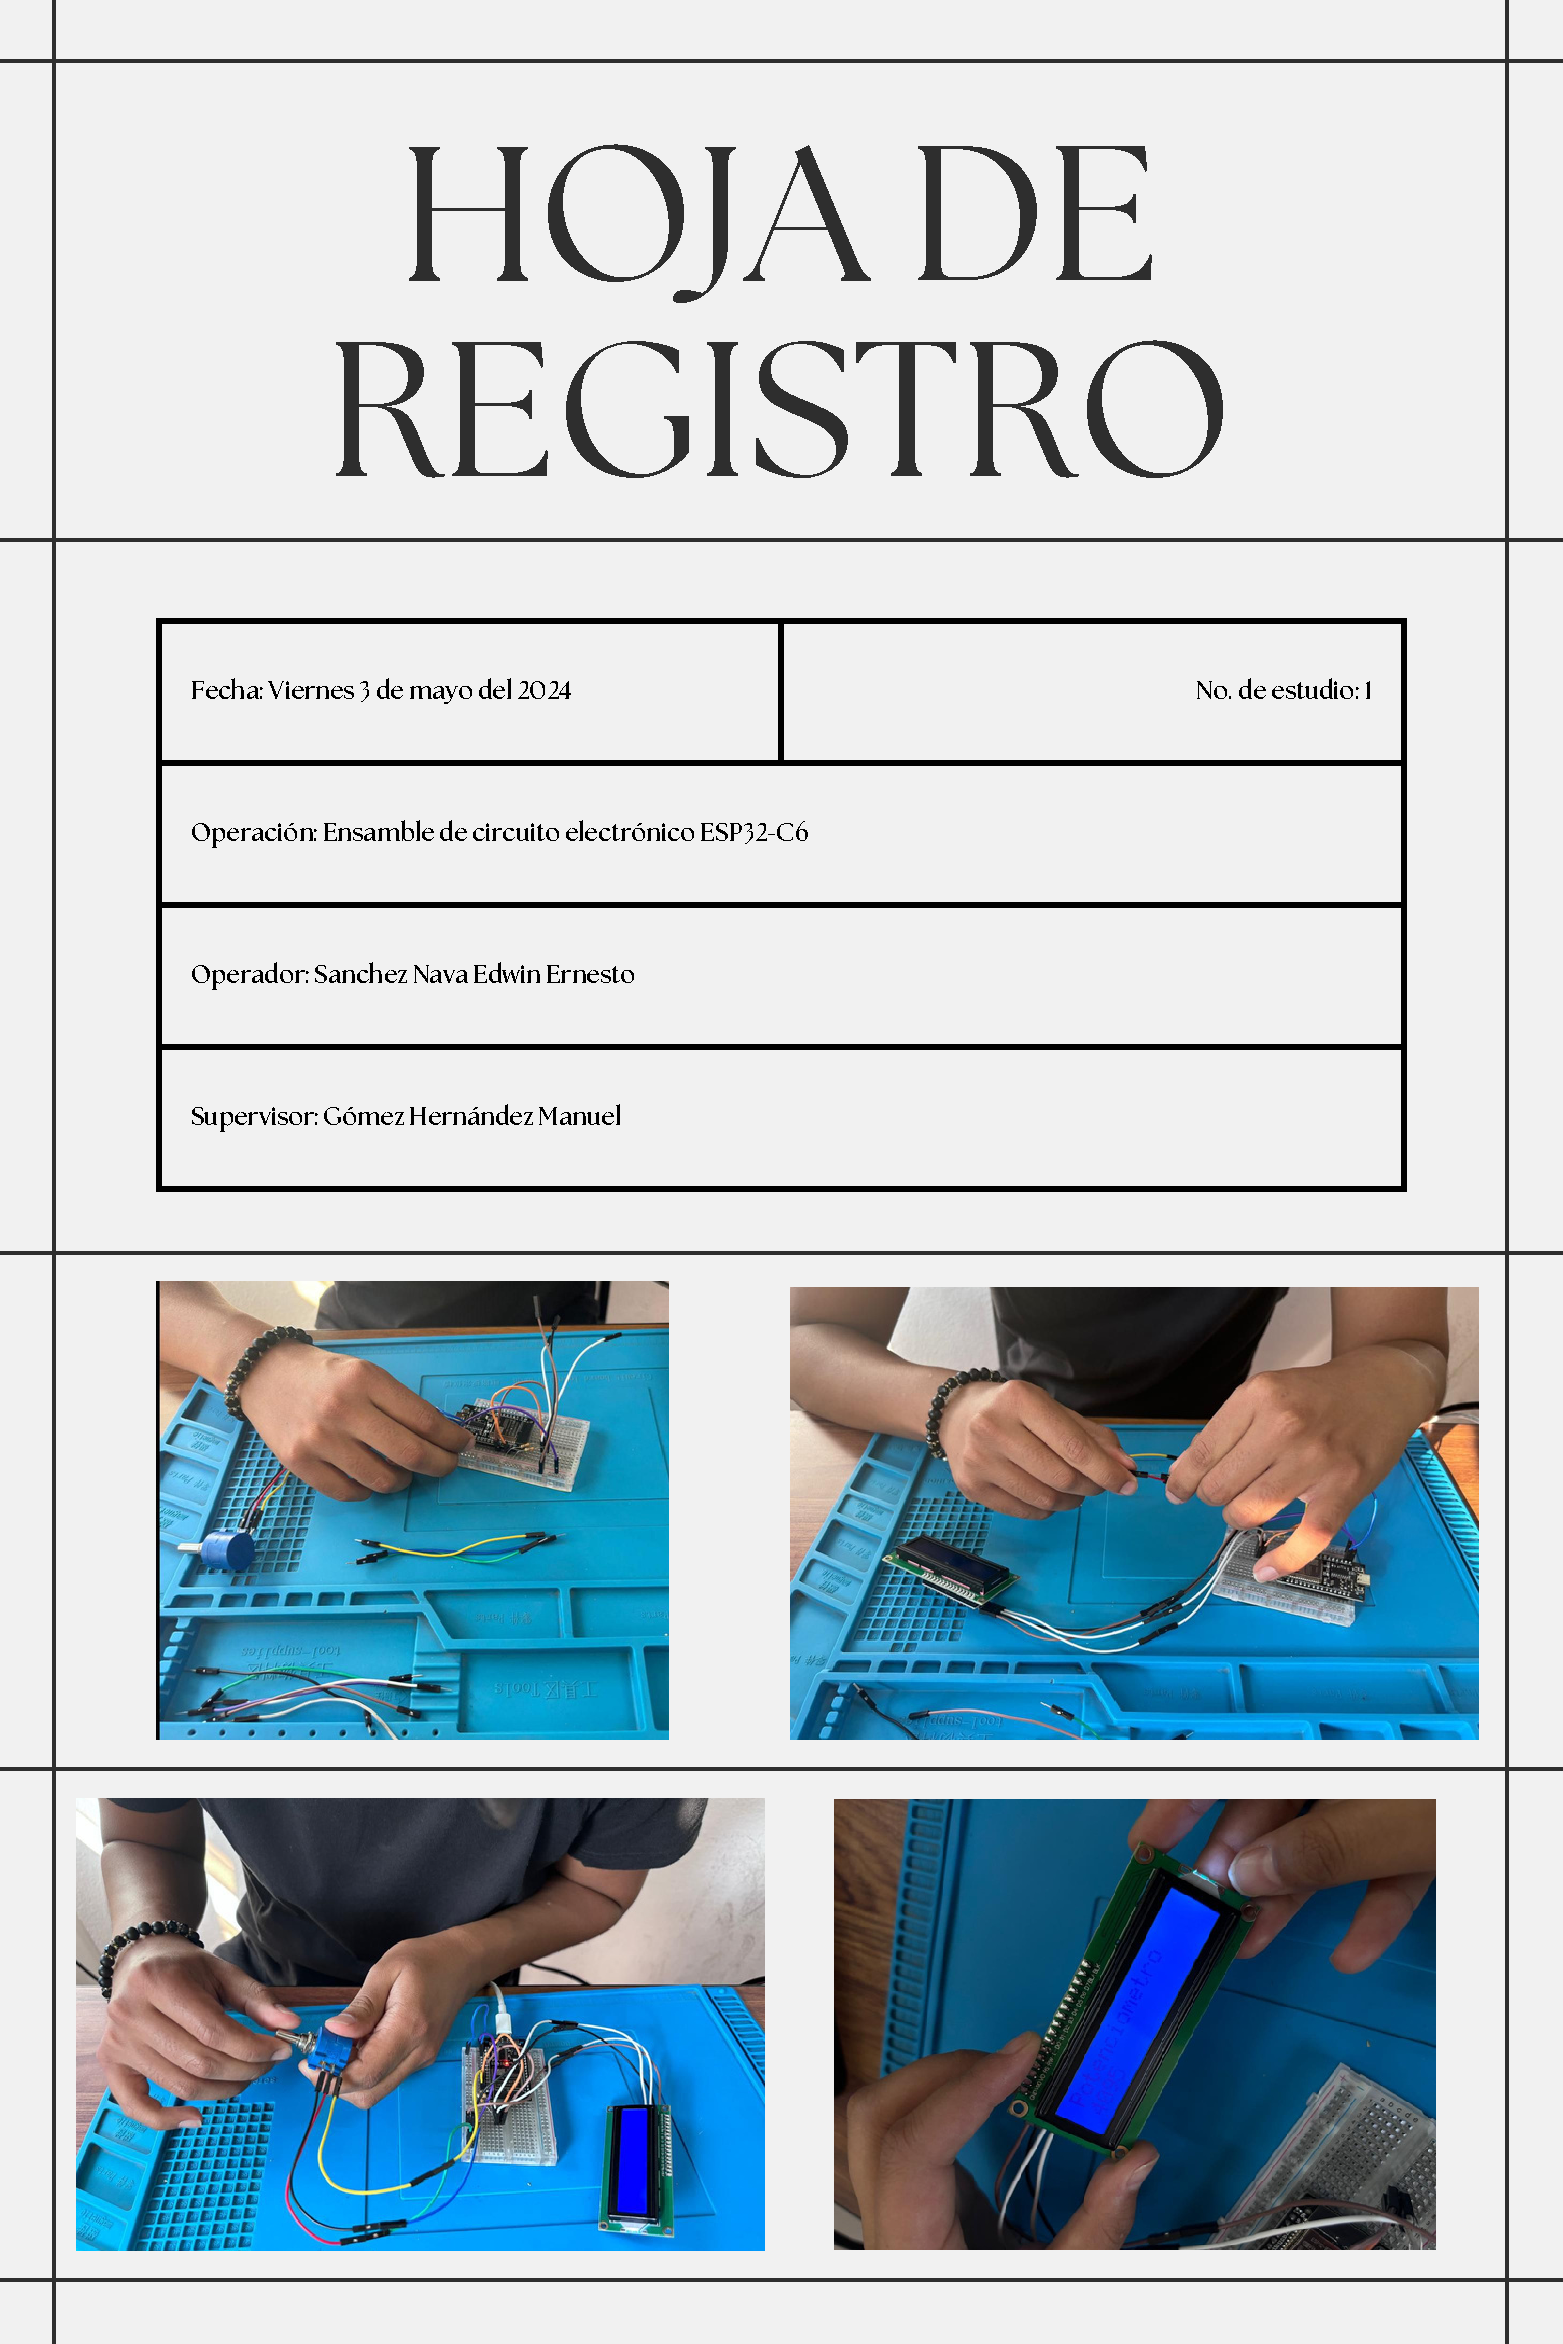
\includepdf[pages=-]{15/img/hojaDeRegistroDeEnsamble.pdf}
    \label{anexo:hojaDeRegistroDeEnsamble.pdf}
    
\newpage
\bibliographystyle{apalike}
\bibliography{15/referencias}

